% This LaTeX document needs to be compiled with XeLaTeX.
\documentclass[10pt]{article}
\usepackage[utf8]{inputenc}
\usepackage{amsmath}
\usepackage{amsfonts}
\usepackage{amssymb}
\usepackage[version=4]{mhchem}
\usepackage{stmaryrd}
\usepackage{bbold}
\usepackage{graphicx}
\usepackage[export]{adjustbox}
\graphicspath{ {./images/} }
\usepackage[fallback]{xeCJK}
\usepackage{polyglossia}
\usepackage{fontspec}
\IfFontExistsTF{Noto Serif CJK TC}
{\setCJKmainfont{Noto Serif CJK TC}}
{\IfFontExistsTF{STSong}
  {\setCJKmainfont{STSong}}
  {\IfFontExistsTF{Droid Sans Fallback}
    {\setCJKmainfont{Droid Sans Fallback}}
    {\setCJKmainfont{SimSun}}
}}

\setmainlanguage{spanish}
\IfFontExistsTF{CMU Serif}
{\setmainfont{CMU Serif}}
{\IfFontExistsTF{DejaVu Sans}
  {\setmainfont{DejaVu Sans}}
  {\setmainfont{Georgia}}
}

\begin{document}
\section*{Capítulo 3 Máximo flujo - Mínimo corte}
\section*{1. Valor del flujo.}
Sea $G=(V, E)$ un grafo dirigido y supongamos que hemos fijado dos vértices $s$ y $t$ a los que llamaremos la fuente y la terminal respectivamente.

Definición 1.1. Si $e \longrightarrow x_{e}$ es una función de $E$ en $\mathbb{R}$, diremos que $x=\left(x_{e}\right)_{e \in E}$ es un flujo en $G$. Además, para cada rama $e=(u, v)$ diremos que $x_{e}=x_{u v}$ es el flujo de la rama $e$.

Sea $x=\left(x_{e}\right)_{e \in E}$ un flujo en $G$.\\
Definición 1.2. Dado un vértice $v$ de $G$ llamaremos\\
flujo que sale de $v$ a

$$
\sum_{w /(v, w) \in E} x_{v w}
$$

flujo que entra en $v$ a

$$
\sum_{w /(w, v) \in E} x_{w v}
$$

flujo neto que sale de $v$ a

$$
\sum_{w /(v, w) \in E} x_{v w}-\sum_{w /(w, v) \in E} x_{w v}
$$

y flujo neto que entra en $v$ a

$$
\sum_{w /(w, v) \in E} x_{w v}-\sum_{w /(v, w) \in E} x_{v w}
$$

Si $A$ y $B$ son subconjuntos de $V$ sea

$$
x(A, B)=\sum_{\substack{v \in A, w \in B \\(v, w) \in E}} x_{v w}
$$

Por abuso de notación, si $v \in V$ escribiremos $x(v, V)$ en lugar de $x(\{v\}, V)$ y $x(V, v)$ en lugar de $x(V,\{v\})$. De esta manera, $x(v, V)$ denota el flujo que sale de $v$ y $x(v, V)-x(V, v)$ el flujo neto que sale de $v$.

Observación 1.3. Si $A \cap B=\emptyset$ entonces

$$
x(A \cup B, C)=x(A, C)+x(B, C)
$$

y

$$
x(C, A \cup B)=x(C, A)+x(C, B)
$$

Lema 1.4. Si el flujo neto que sale de $v$ es nulo para todo $v \neq s, t$ entonces el flujo neto que sale de $s$ es igual al flujo neto que entra en $t$.\\
Demostración: Sabemos que $x(v, V)-x(V, v)=0 \forall v \neq s, t$. Veamos que $x(s, V)-x(V, s)=x(V, t)-x(t, V)$. Por la observación 1.3. se tiene que

$$
x(V, V)=x(s, V)+x(t, V)+\sum_{v \neq s, t} x(v, V)
$$

y

$$
x(V, V)=x(V, s)+x(V, t)+\sum_{v \neq s, t} x(V, v)
$$

Luego,

$$
0=x(V, V)-x(V, V)=x(s, V)-x(V, s)+x(t, V)-x(V, t)+\sum_{v \neq s, t} x(v, V)-x(V, v)
$$

de donde $x(s, V)-x(V, s)=x(V, t)-x(t, V)$ como queríamos probar.\\
Definición 1.5. Diremos que un flujo ( $x_{e}$ ) es un $b$-flujo (balanced flow) si satisface las hipótesis del lema 1.4. (i.e., si el flujo neto que sale de $v$ es nulo para todo $v \neq s, t$ ). En tal caso llamaremos valor del flujo al flujo neto que sale de $s$.\\
Ejemplo 1.6. Consideremos en el siguiente grafo el flujo $x_{e}$ indicado en cada rama $e$\\
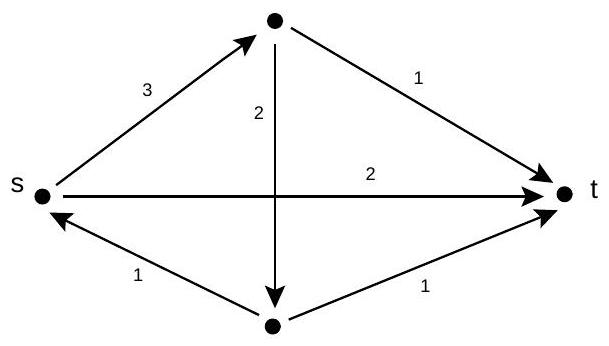
\includegraphics[max width=\textwidth, center]{2025_09_05_aa5f7b8425e7dd302062g-02}

Este flujo satisface las hipótesis del lema 1.4. En este caso el valor del flujo es 4.

\section*{2. El problema del máximo flujo.}
Sea $G=(V, E)$ un grafo dirigido donde hemos fijado dos vértices $s$ y $t$ a los que llamaremos la fuente y la terminal respectivamente. Supondremos además que algunas ramas $e=(v, w)$ tienen asignado un número real positivo $u_{e}=u_{v w}$ al que llamaremos capacidad de la rama e. A las ramas que no tengan restricción de capacidades asignamos capacidad infinita. Luego, cada $e \in E$ tiene asignado un valor $u_{e}$ tal que $0<u_{e} \leq \infty (e \in E)$.

Describiremos un algoritmo para resolver el siguiente problema:\\
Encontrar un b-flujo $\left(x_{e}\right)_{e \in E}$ tal que el valor del flujo sea máximo sujeto a la restricción de que el flujo de cada rama sea no negativo y no exceda su capacidad, es decir, queremos resolver

$$
\begin{aligned}
& \max x(s, V)-x(V, s) \\
& x(v, V)-x(V, v)=0 \quad \forall v \neq s, t \\
& 0 \leq x_{e} \leq u_{e} \quad(e \in E)
\end{aligned}
$$

Observemos que este es un problema de programación lineal. En efecto, es el problema

$$
\begin{aligned}
& \max \sum_{w /(s, w) \in E} x_{s w}-\sum_{w /(w, s) \in E} x_{w s} \\
& \sum_{w /(v, w) \in E} x_{v w}-\sum_{w /(w, v) \in E} x_{w v}=0 \quad \forall v \neq s, t \\
& \quad 0 \leq x_{v w} \leq u_{v w}
\end{aligned}
$$

y, por lo tanto, lo podríamos resolver aplicando el algoritmo simplex. La ventaja sobre el simplex que tiene el algoritmo que veremos es que produce soluciones enteras cuando los datos son enteros.

Describiremos ahora el algoritmo de Ford-Fulkerson, que utilizará ciertos caminos de $s$ a $t$ que llamaremos caminos aumentativos. Si $\mathcal{P}$ es un camino y $e \in E$ escribiremos por abuso de notación $e \in \mathcal{P}$ para significar que $e$ es una rama del camino $\mathcal{P}$.

Dado $v \in V$, si $\mathcal{P}$ es un camino de $s$ a $v$ y $e \in \mathcal{P}$, diremos que $e$ tiene la dirección $s \longrightarrow v$ o también que $e$ es directa si al recorrer $\mathcal{P}$ desde $s$ hacia $v$ pasamos por la cola de $e$ antes que por la punta.\\
Análogamente diremos que $e$ tiene la dirección $s \longleftarrow v$ o también que e es inversa si al recorrer $\mathcal{P}$ desde $s$ hacia $v$ pasamos por la punta de $e$ antes que por la cola.

Ejemplo 2.1. En el camino de $s$ a $t$\\
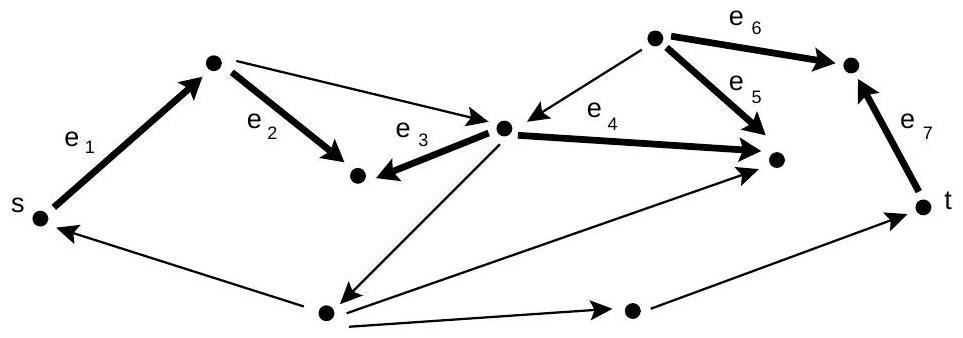
\includegraphics[max width=\textwidth, center]{2025_09_05_aa5f7b8425e7dd302062g-03}\\
$\mathcal{P}=\left(e_{1}, e_{2}, e_{3}, e_{4}, e_{5}, e_{6}, e_{7}\right)$ las ramas $e_{1}, e_{2}, e_{4}$ y $e_{6}$ son directas y las ramas $e_{3}, e_{5}$ y $e_{7}$ son inversas.\\
Observación 2.2. Supongamos que tenemos en $G$ un flujo ( $x_{e}$ ) factible, es decir, tal que $x(v, V)-x(V, v)=0 \forall v \neq s, t$ y $0 \leq x_{e} \leq u_{e} \forall e \in E$. Si $\mathcal{P}$ es un camino simple en $G$ de $s$ a $t$ tal que

$$
x_{e}<u_{e} \quad \forall e \in \mathcal{P} \text { con dirección } s \longrightarrow t
$$

y

$$
0<x_{e} \quad \forall e \in \mathcal{P} \text { con dirección } s \longleftarrow t
$$

Tomando $\delta>0$ tal que

$$
\delta \leq \min \left\{u_{e}-x_{e} / e \in \mathcal{P} \text { con dirección } s \longrightarrow t\right\}
$$

y

$$
\delta \leq \min \left\{x_{e} / e \in \mathcal{P} \text { con dirección } s \longleftarrow t\right\}
$$

sumando $\delta$ a cada $x_{e}$ tal que $e \in \mathcal{P}$ tiene dirección $s \longrightarrow t$ y restando $\delta$ a cada $x_{e}$ tal que $e \in \mathcal{P}$ tiene dirección $s \longleftarrow t$, obtendremos un nuevo flujo $x^{\prime}=\left(x_{e}^{\prime}\right)$ que también será factible y cuyo valor de flujo será igual al valor del flujo $x=\left(x_{e}\right)$ más $\delta$. Es decir, tomando

$$
x_{e}^{\prime}= \begin{cases}x_{e}+\delta & \text { si } e \in \mathcal{P} \text { es directa } \\ x_{e}-\delta & \text { si } e \in \mathcal{P} \text { es inversa } \\ x_{e} & \text { si } e \notin \mathcal{P}\end{cases}
$$

resulta que $x^{\prime}$ es factible y

$$
\text { valor del flujo } x^{\prime}=\delta+\text { valor del flujo } x
$$

Definición 2.3. Sea $x=\left(x_{e}\right)$ un flujo en $G$ y sea $v$ un vértice distinto de $s$. Diremos que un camino simple $\mathcal{P}$ de $s$ a $v$ es un camino aumentativo de $x$ (o simplemente que $\mathcal{P}$ es un camino aumentativo cuando no haya duda de cuál es el flujo $x$ del que se trata) sii

$$
x_{e}<u_{e} \quad \forall e \in \mathcal{P} \text { que tiene dirección } s \longrightarrow v
$$

y

$$
0<x_{e} \quad \forall e \in \mathcal{P} \text { que tiene dirección } s \longleftarrow v
$$

Por la observación 2.2., si $x$ es un flujo factible y $\mathcal{P}$ es un camino aumentativo de $s$ a $t$ entonces podemos encontrar un flujo factible $x^{\prime}$ con mayor valor de flujo que $x$.\\
Ejemplo 2.4. Consideremos el siguiente grafo, donde para cada rama $e$ se indica el flujo $x_{e}$ y también, entre paréntesis, la capacidad $u_{e}$.\\
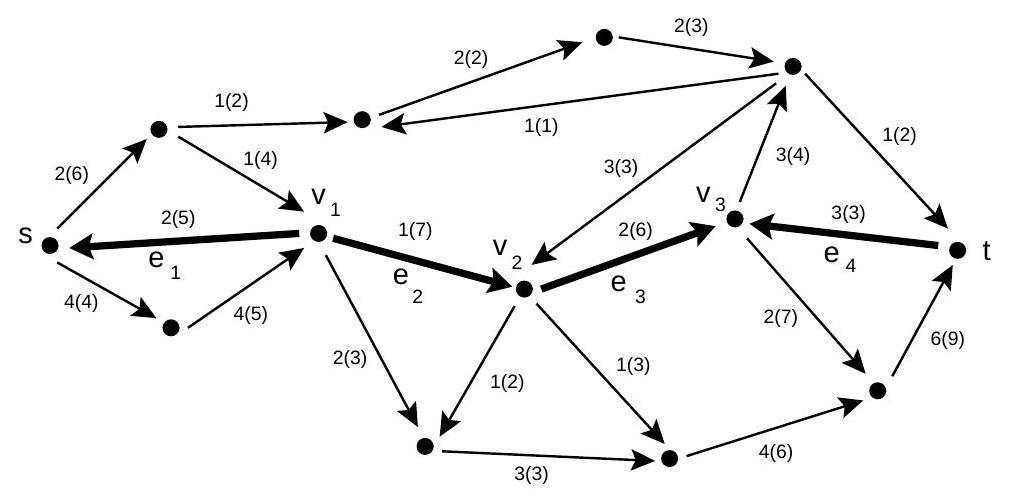
\includegraphics[max width=\textwidth, center]{2025_09_05_aa5f7b8425e7dd302062g-04(1)}

Dejamos como tarea al lector comprobar que el flujo $x$ es factible, con valor 4 y que el camino marcado con trazo grueso es un camino aumentativo de $s$ a $t$ que nos permitiría aumentar el flujo en $\delta=2$. En este camino, las ramas $e_{2}$ y $e_{3}$ tienen la dirección $s \longrightarrow t$ y las ramas $e_{1}$ y $e_{4}$ tienen la dirección $s \longleftarrow t$. Si sumamos $\delta=2$ al flujo de las ramas directas y restamos $\delta=2$ al flujo de las ramas inversas obtenemos el nuevo flujo

$$
x_{e}^{\prime}= \begin{cases}x_{e}+\delta & \text { si } e=e_{2}, e_{3} \\ x_{e}-\delta & \text { si } e=e_{1}, e_{4} \\ x_{e} & \text { si } e \neq e_{1}, e_{2}, e_{3}, e_{4}\end{cases}
$$

\begin{center}
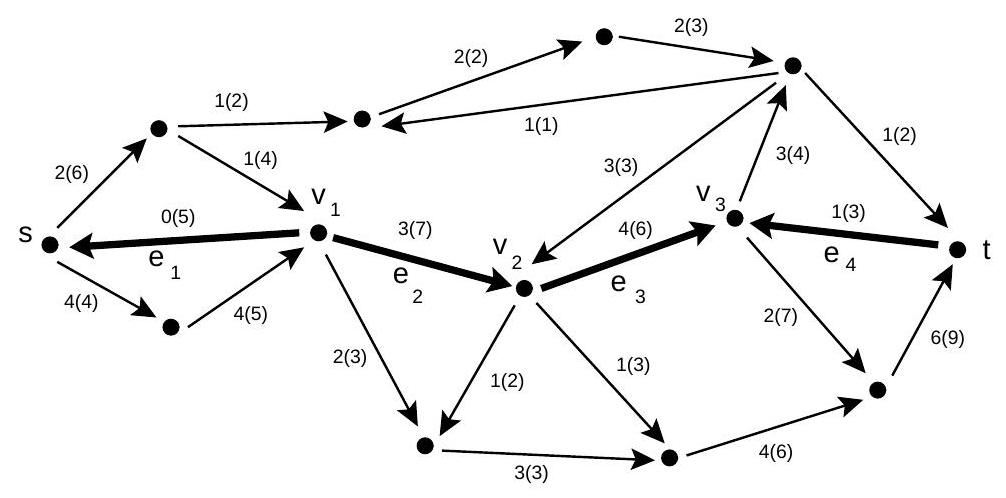
\includegraphics[max width=\textwidth]{2025_09_05_aa5f7b8425e7dd302062g-04}
\end{center}

Este nuevo flujo es factible pues como $0 \leq x_{e} \leq u_{e} \forall e \in E$ y $\delta>0$ satisface

$$
\delta \leq \min \left\{u_{e_{2}}-x_{e_{2}}, u_{e_{3}}-x_{e_{3}}\right\} \quad y \quad \delta \leq \min \left\{x_{e_{1}}, x_{e_{4}}\right\}
$$

entonces $0 \leq x_{e_{1}}-\delta \leq u_{e_{1}}, 0 \leq x_{e_{2}}+\delta \leq u_{e_{2}}, 0 \leq x_{e_{3}}+\delta \leq u_{e_{3}}$ y $0 \leq x_{e_{4}}-\delta \leq u_{e_{4}}$.\\
Luego $x^{\prime}$ verifica $0 \leq x_{e}^{\prime} \leq u_{e}(e \in E)$. Además, $x^{\prime}$ es un b-flujo. En efecto, el flujo neto que sale de cada vértice $v \neq s, t$ no se ha modificado ya que cada $\delta$ que se suma se compensa con uno que se resta:

$$
\begin{aligned}
& x^{\prime}\left(v_{1}, V\right)-x^{\prime}\left(V, v_{1}\right)=x_{e_{1}}^{\prime}+x_{e_{2}}^{\prime}+2-1-4=x_{e_{1}}-\delta+x_{e_{2}}+\delta+2-1-4= \\
& \quad=x_{e_{1}}+x_{e_{2}}+2-1-4=x\left(v_{1}, V\right)-x\left(V, v_{1}\right)=0 \\
& x^{\prime}\left(v_{2}, V\right)-x^{\prime}\left(V, v_{2}\right)=x_{e_{3}}^{\prime}+1+1-x_{e_{2}}^{\prime}-3=x_{e_{3}}+\delta+1+1-\left(x_{e_{2}}+\delta\right)-3= \\
& =x_{e_{3}}+1+1-x_{e_{2}}-3=x\left(v_{2}, V\right)-x\left(V, v_{2}\right)=0
\end{aligned}
$$

$$
\begin{aligned}
& x^{\prime}\left(v_{3}, V\right)-x^{\prime}\left(V, v_{3}\right)=3+2-x_{e_{3}}^{\prime}-x_{e_{4}}^{\prime}=3+2-\left(x_{e_{3}}+\delta\right)-\left(x_{e_{4}}-\delta\right)= \\
& \quad=3+2-x_{e_{3}}-x_{e_{4}}=x\left(v_{3}, V\right)-x\left(V, v_{3}\right)=0
\end{aligned}
$$

y, claramente, si $v \neq v_{1}, v_{2}, v_{3}$ entonces $x^{\prime}(v, V)-x^{\prime}(V, v)=x(v, V)-x(V, v)=0$.\\
Verifiquemos que el valor del flujo aumentó en $\delta$ :

$$
\begin{aligned}
& x^{\prime}(s, V)-x^{\prime}(V, s)=2+4-x_{e_{1}}^{\prime}=2+4-\left(x_{e_{1}}-\delta\right)= \\
& 2+4-x_{e_{1}}+\delta=x(s, V)-x(V, s)+\delta
\end{aligned}
$$

Ahora repetimos el procedimiento. Partiendo del flujo\\
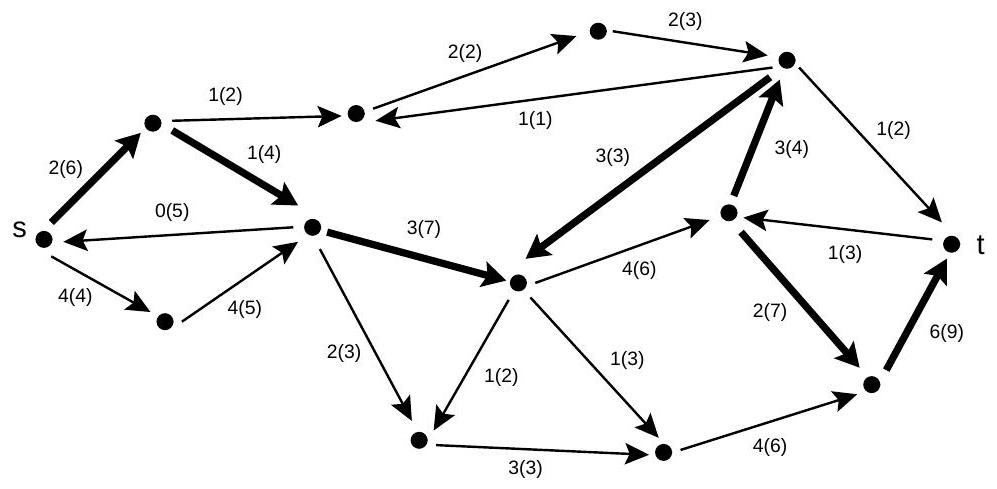
\includegraphics[max width=\textwidth, center]{2025_09_05_aa5f7b8425e7dd302062g-05(1)}\\
y usando el camino aumentativo de $s$ a $t$ indicado con trazo grueso podemos volver a aumentar el valor del flujo en $\delta=3$. En este camino la cuarta y quinta ramas son inversas y las restantes ramas son directas. Luego el nuevo flujo será\\
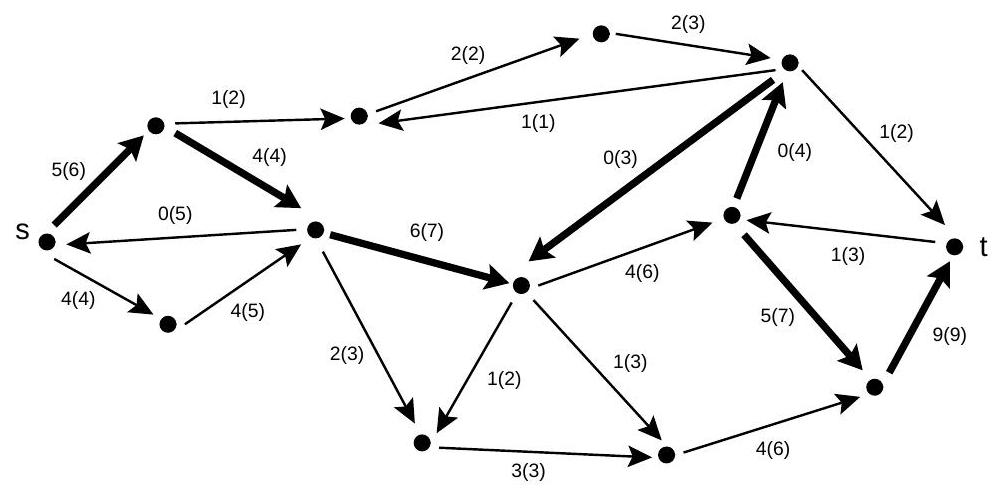
\includegraphics[max width=\textwidth, center]{2025_09_05_aa5f7b8425e7dd302062g-05}

Verifiquemos que el valor del flujo aumentó en $\delta$ :

$$
x^{\prime}(s, V)-x^{\prime}(V, s)=5+4=9=6+3=6+\delta
$$

\section*{Esquema del algoritmo de Ford-Fulkerson.}
\begin{enumerate}
  \item $x=x_{0}$, donde $x_{0}$ es cualquier flujo factible inicial (por ejemplo, $x_{0}=0$ ).
  \item buscar un camino aumentativo de $x$ de $s$ a $t$. Si no existe, STOP.
  \item Actualizar $x$ sumando o restando $\delta$ al flujo de las ramas del camino aumentativo según la dirección, en la forma indicada en la observación 2.2., para obtener un flujo de mayor valor.
  \item goto 2.
\end{enumerate}

En la sección 4. veremos este algoritmo en detalle. Daremos condiciones que garantizan un STOP (en principio, este algoritmo podría no detenerse nunca) y probaremos que si en alguna iteración no existe un camino aumentativo de $x$ de $s$ a $t$ entonces el flujo $x$ presente en ese momento es máximo.

\section*{3. El problema del mínimo corte.}
Sea $G=(V, E)$ un grafo dirigido con fuente $s$ y terminal $t$ y donde cada rama $e=(v, w) \in E$ tiene asignada una capacidad $u_{e}=u_{v w}$, donde $0<u_{e} \leq \infty$.

Recordemos que si $A$ es un subconjunto del conjunto de vértices del grafo dirigido $G$, el corte definido por $A$ es el conjunto

$$
\partial A=\{(v, w) \in E / v \in A \wedge w \notin A\}
$$

De ahora en más sólo consideraremos cortes definidos por conjuntos $A$ que contengan a la fuente y no a la terminal, es decir, tales que $s \in A$ y $t \notin A$. Denotaremos por $\bar{A}$ al complemento de $A$ respecto de $V$.

Definición 3.1. Sea $\partial A$ un corte tal que $s \in A$ y $t \notin A$. Definimos la capacidad del corte $\partial A$ como la suma de las capacidades de las ramas del corte, es decir,

$$
u(A, \bar{A})=\sum_{e \in \partial A} u_{e}=\sum_{\substack{v \in A, w \in \bar{A} \\(v, w) \in E}} u_{v w}
$$

Consideremos el problema del máximo flujo

$$
\begin{aligned}
& \max x(s, V)-x(V, s) \\
& x(v, V)-x(V, v)=0 \quad \forall v \neq s, t \\
& 0 \leq x_{e} \leq u_{e} \quad(e \in E)
\end{aligned}
$$

Como siempre, diremos que un flujo $x$ en $G$ es factible si satisface las restricciones del problema. Veremos que el problema del máximo flujo tiene como dual al problema del mínimo corte que consiste en hallar un corte $\partial A$ de mínima capacidad entre todos los cortes definidos por conjuntos que contienen a $s$ y no a $t$. Para probar esto necesitaremos antes algunos resultados.

Lema 3.2. Sea $x=\left(x_{e}\right)$ un flujo factible en $G$, es decir, tal que $x(v, V)-x(V, v)=0 \forall v \neq s, t$ y $0 \leq x_{e} \leq u_{e} \forall e \in E$. Sea $\partial A$ un corte tal que $s \in A$ y $t \notin A$. Entonces

$$
x(s, V)-x(V, s)=x(A, \bar{A})-x(\bar{A}, A)
$$

\section*{Demostración:}
$$
x(A, V)-x(V, A)=x(s, V)-x(V, s)+\sum_{v \in A-\{s\}} x(v, V)-x(V, v)
$$

Como $x(v, V)-x(V, v)=0$ para todo $v \neq s, t$ y $t \notin A$ entonces $x(v, V)-x(V, v)=0$ para todo $v \in A-\{s\}$. Luego, $x(A, V)-x(V, A)=x(s, V)-x(V, s)$. Siendo que $V$ es la unión disjunta de $A$ y $\bar{A}$, por la observación 1.3. se tiene que

$$
\begin{aligned}
& x(A, V)-x(V, A)=x(A, A \cup \bar{A})-x(A \cup \bar{A}, A)= \\
& =x(A, A)+x(A, \bar{A})-x(A, A)-x(\bar{A}, A)=x(A, \bar{A})-x(\bar{A}, A)
\end{aligned}
$$

Luego, $x(s, V)-x(V, s)=x(A, \bar{A})-x(\bar{A}, A)$. .

Corolario 3.3. Sea $x=\left(x_{e}\right)$ un flujo factible y sea $\partial A$ un corte tal que $s \in A$ y $t \notin A$. Entonces el valor del flujo $x$ es menor o igual que la capacidad del corte $\partial A$, es decir,

$$
x(s, V)-x(V, s) \leq u(A, \bar{A})
$$

Demostración: Como $x(A, \bar{A}) \geq 0$ pues $x$ es factible, por el lema 3.2. se tiene que

$$
\begin{aligned}
& x(s, V)-x(V, s)=x(A, \bar{A})-x(\bar{A}, A) \leq x(A, \bar{A})= \\
& =\sum_{\substack{v \in A, w \in \bar{A} \\
(v, w) \in E}} x_{v w} \leq \sum_{\substack{v \in A, w \in \bar{A} \\
(v, w) \in E}} u_{v w}=u(A, \bar{A})
\end{aligned}
$$

Por lo tanto $x(s, V)-x(V, s) \leq u(A, \bar{A})$. ㅁ\\
Lema 3.4. Sea $x$ un flujo factible tal que no existe camino aumentativo de $x$ de $s$ a $t$. Sea $A$ el conjunto que contiene a $s$ pero no a $t$ definido por

$$
A=\{s\} \cup\{v \in V / \text { existe un camino aumentativo de } x \text { de } s \text { a } v\}
$$

Entonces la capacidad del corte $\partial A$ es igual al valor del flujo $x$.\\
Demostración: Sea $x$ un flujo factible tal que no existe camino aumentativo de $x$ de $s$ a $t$. Sea $A=\{s\} \cup\{v \in V /$ existe un camino aumentativo de $x$ de $s$ a $v\}$.\\
Veamos que la capacidad de $\partial A$ es igual al valor de $x$.\\
Sean $v \in A$ y $w \in \bar{A}$. Entonces hay un camino aumentativo de $s$ a $v$ y no lo hay de $s$ a $w$. Luego, si $e=(v, w) \in E$ entonces $x_{e}=u_{e}$. En efecto, si fuese $x_{e}<u_{e}$ entonces el camino aumentativo que va de $s$ a $v$ seguido de la rama ( $v, w$ ) sería un camino aumentativo de $s$ a $w$. Análogamente, si $e=(w, v) \in E$ entonces debe ser $x_{e}=0$. En otras palabras, en las ramas que tienen la cola en $A$ y la punta en $\bar{A}$ el flujo es igual a la capacidad de la rama mientras que en las que tienen la cola en $\bar{A}$ y la punta en $A$ el flujo es nulo. Luego,

$$
x(A, \bar{A})-x(\bar{A}, A)=u(A, \bar{A})-0=u(A, \bar{A})
$$

Pero por el lema 3.2. $x(A, \bar{A})-x(\bar{A}, A)=x(s, V)-x(V, s)$, por lo tanto el valor del flujo $x$ es igual a la capacidad del corte $\partial A$. 口

Ahora sí probemos el teorema de dualidad.\\
Teorema 3.5. (max flow - min cut) Si $x$ es un flujo óptimo (es decir, un flujo factible de valor máximo) entonces el corte $\partial A$ definido por el conjunto $A$ del lema 3.4. es un mínimo corte (es decir, $\partial A$ tiene capacidad mínima entre los cortes definidos por conjuntos que contienen a $s$ y no a $t$ ) y su capacidad es igual al valor del flujo $x$.\\
Demostración: Sea $x$ un flujo factible de valor máximo. Si existiera un camino aumentativo de $x$ de $s$ a $t$ entonces, por la observación 2.2., podríamos aumentar el valor de $x$. Luego no existe un camino aumentativo de $s$ a $t$. Por lo tanto, por el lema 3.4. el corte $\partial A$ tiene capacidad igual al valor del flujo $x$.\\
Si $\partial B$ es un corte tal que $s \in B$ y $t \notin B$ entonces, por el corolario 3.3., el valor de $x$ es menor o igual que la capacidad de $\partial B$, de donde

$$
\text { capacidad de } \partial A=\text { valor de } x \leq \text { capacidad de } \partial B
$$

Luego $\partial A$ es un corte de capacidad mínima entre los cortes definidos por conjuntos que contienen a $s$ y no a $t$ y su capacidad es igual al valor del flujo $x$. ㅁ

En la próxima sección describiremos el algoritmo de Ford-Fulkerson con más detalle y mostraremos que este algoritmo encuentra el mínimo corte cuando resuelve el problema de máximo flujo (es decir, cuando el algoritmo resuelve el problema del máximo flujo obtiene también la solución al problema dual del mínimo corte).

\section*{4. El algoritmo de Ford-Fulkerson.}
Sea $G=(V, E)$ un grafo dirigido con fuente $s$ y terminal $t$ y sea $0<u_{e} \leq \infty$ la capacidad de la rama $e (e \in E)$ y consideremos el problema del máximo flujo

$$
\begin{aligned}
& \max x(s, V)-x(V, s) \\
& x(v, V)-x(V, v)=0 \quad \forall v \neq s, t \\
& 0 \leq x_{e} \leq u_{e} \quad(e \in E)
\end{aligned}
$$

Proposición 4.1. Sea $x$ un flujo factible. Entonces $x$ es óptimo sii no existe un camino aumentativo de $x$ de $s$ a $t$.\\
Demostración: $(\Longrightarrow)$ es trivial.\\
$(\Longleftarrow)$ Sea $x$ un flujo factible. Si no existe un camino aumentativo de $x$ de $s$ a $t$ entonces, por el lema 3.4. existe un corte $\partial A$ tal que $s \in A$ y $t \notin A$ cuya capacidad es igual al valor del flujo $x$. Luego el flujo debe ser óptimo. En efecto, si $x^{\prime}$ es un flujo factible entonces, por el corolario 3.3.,

$$
\text { valor de } x^{\prime} \leq \text { capacidad de } \partial A=\text { valor de } x \text { ㅁ }
$$

Proposición 4.2. Si $u$ es entero (es decir, que $u_{e} \in \mathbb{Z}$ para todo $e \in E$ ) entonces existe un flujo óptimo $x$ que además es entero (es decir, satisface $x_{e} \in \mathbb{Z}$ para toda rama $e$ ).\\
Demostración: El conjunto de todos los flujos $x$ que son factibles y enteros es no vacío (pues $x_{e}=0 \forall e \in E$ es un flujo factible que es entero) y finito (si $x$ es un flujo factible entero entonces, para cada $e \in E, x_{e}$ puede tomar a lo sumo los $u_{e}+1$ valores $0,1,2, \ldots u_{e}$ ). Sea $x$ un flujo de valor máximo en este conjunto. Basta ver que $x$ es óptimo.\\
Supongamos que existiera un camino aumentativo de $x$ de $s$ a $t$. Entonces, como $u$ y $x$ son enteros podríamos aumentar el flujo en un $\delta$ entero (ver observación 2.2.) y así encontrar un flujo factible entero de mayor valor que $x$, cosa que contradice la elección de $x$. Luego, no existe camino aumentativo de $s$ a $t$ y por lo tanto, por la proposición 4.1. resulta que $x$ es óptimo. -

Describiremos ahora en más detalle el algoritmo para hallar un flujo óptimo. Veremos que este algoritmo resuelve el problema de máximo flujo al mismo tiempo que el problema del mínimo corte. En cada iteración del algoritmo se tendrá un flujo factible $x$ (tomaremos $x=0$ como flujo factible inicial) a partir del cual se construirá el conjunto

$$
A=\{s\} \cup\{v \in V / \text { existe un camino aumentativo de } x \text { de } s \text { a } v\}
$$

del lema 3.4. Una vez hallado el conjunto $A$ correspondiente al flujo $x$ de la presente iteración, si $t \notin A$ el algoritmo se detendrá. Como $t \notin A$ entonces no existe camino aumentativo de $s$ a $t$ y por lo tanto el flujo $x$ de la presente iteración es óptimo por la proposición 4.1. Dado que $x$ es óptimo entonces el corte definido por el último conjunto $A$ generado por el algoritmo (que fue construído a partir de $x$ ) resulta mínimo (ver teorema 3.5.).\\
En cambio, si $t \in A$ entonces existe un camino aumentativo $\mathcal{P}$ de $s$ a $t$. Si todas las ramas de ese camino son directas y de capacidad infinita entonces el algoritmo se detendrá. En este caso es posible aumentar el valor\\
del flujo tanto como se quiera, es decir, no existe un flujo de valor máximo. En el caso en que el camino $\mathcal{P}$ contenga ramas inversas o ramas directas de capacidad finita, supongamos que conocemos las ramas de ese camino, su dirección y $\delta$ tal que

$$
\delta \leq \min \left\{u_{e}-x_{e} / e \in \mathcal{P} \text { es directa }\right\} \quad \text { y } \quad \delta \leq \min \left\{x_{e} / e \in \mathcal{P} \text { es inversa }\right\}
$$

Entonces el flujo $x^{\prime}$ obtenido sumando $\delta$ a cada $x_{e}$ tal que $e \in \mathcal{P}$ es directa y restando $\delta$ a cada $x_{e}$ tal que $e \in \mathcal{P}$ es inversa, es factible y el valor de $x^{\prime}=$ valor de $x+\delta$. En ese caso reemplazamos el flujo $x$ por $x^{\prime}$ y hacemos una nueva iteración.\\
Ahora veamos cómo hacer para poder determinar, cuando $t \in A$, las ramas del camino aumentativo de $s$ a $t$, su dirección y el $\delta$ que nos permitirá actualizar el flujo para comenzar una nueva iteración. Para lograr esto, como buscamos un conjunto $A$ que contenga a $s$ comenzamos ingresando $s$ en $A$ y poniendo $\delta(s)=\infty$. Luego, al ingresar cada $w$ en $A$ (notemos que como lo que queremos es construír

$$
A=\{s\} \cup\{v \in V / \text { existe un camino aumentativo de } x \text { de } s \text { a } v\}
$$

entonces ingresaremos $w$ en $A$ cuando haya un camino aumentativo $\mathcal{C}$ de $s$ a $w$ ) le adjuntaremos la terna $(p(w), s g(w), \delta(w))$ donde $p(w)$ será el vértice anterior a $w$ en el camino aumentativo $\mathcal{C}$ de $s$ a $w, s g(w)=1$ si la última rama en $\mathcal{C}$ (es decir, la rama que une $p(w)$ y $w$ ) es directa y $s g(w)=-1$ si es inversa y $\delta(w)>0$ satisfacerá

$$
\begin{aligned}
& \delta(w) \leq \min \left\{u_{e}-x_{e} / e \in \mathcal{C} \text { es directa }\right\} \\
& \delta(w) \leq \min \left\{x_{e} / e \in \mathcal{C} \text { es inversa }\right\}
\end{aligned}
$$

Llamaremos a $(p(w), s g(w), \delta(w))$ la etiqueta de $w$.\\
En cada iteración ingresaremos algunos $w \notin A$ tales que existe un camino aumentativo de $s$ a $w$. Observemos que si para algún $v$ tal que existe un camino aumentativo de $s$ a $v$ (por ejemplo, para un $v$ ingresado a $A$ en una iteración anterior) ocurre que $(v, w) \in E$ o $(w, v) \in E$ entonces el camino aumentativo de $s$ a $v$ se puede extender a un camino de $s$ a $w$ que será aumentativo o no de acuerdo a cómo sea el flujo en esa última rama. Más precisamente, si $v \in A,(v, w) \in E$ (es decir, si $(v, w) \in \partial A)$ y $x_{v w}<u_{v w}$ entonces el camino aumentativo de $s$ a $v$ seguido de la rama ( $v, w$ ) resulta un camino aumentativo de $s$ a $w$, la última rama es directa, el predecesor a $w$ en ese camino es $v$ y el máximo $\delta(w)$ que podemos tomar es $\min \left\{\delta(v), u_{v w}-x_{v w}\right\}$. Entonces ingresamos $w$ en $A$, ponemos $p(w)=v, s g(w)=1$ y $\delta(w)=\min \left\{\delta(v), u_{v w}-x_{v w}\right\}$.\\
Pero si en cambio $v \in A,(w, v) \in E$ (es decir, $(w, v) \in \partial \bar{A}$ ) y $x_{w v}>0$ entonces el camino aumentativo de $s$ a $v$ seguido de la rama ( $w, v$ ) resulta un camino aumentativo de $s$ a $w$, la última rama es inversa, el predecesor a $w$ en ese camino es $v$ y el máximo $\delta(w)$ que podemos tomar es $\min \left\{\delta(v), x_{w v}\right\}$.\\
En este caso ingresamos $w$ en $A$, ponemos $p(w)=v, s g(w)=-1$ y $\delta(w)=\min \left\{\delta(v), x_{w v}\right\}$.\\
Observemos que en ambos casos $\delta(v)>0$ implica $\delta(w)>0$ y como $\delta(s)=\infty>0$ entonces $\delta(u)>0$ para todo $u \in A$.\\
Luego, $A$ es construído de forma tal que para cada $v \in A$ valga $p(v) \in A$. Por lo tanto, si $t \in A$, podremos reconstruír el camino aumentativo de $s$ a $t$ utilizando $p:$ si

$$
p(t)=w_{1}, p\left(w_{1}\right)=w_{2}, \ldots, p\left(w_{n-1}\right)=w_{n}, p\left(w_{n}\right)=s
$$

entonces el camino aumentativo de $s$ a $t$ es $\left(s, w_{n}, w_{n-1}, \ldots, w_{2}, w_{1}, t\right)$.\\
Además, $s g\left(w_{n}\right)$ nos dirá la dirección de la rama que une $s=p\left(w_{n}\right)$ y $w_{n}, s g\left(w_{n-1}\right)$ la de la rama que une $w_{n}=p\left(w_{n-1}\right)$ y $w_{n-1}, \ldots, s g\left(w_{1}\right)$ la de la rama que une $w_{2}=p\left(w_{1}\right)$ y $w_{1}$ y $s g(t)$ la de la rama que une $w_{1}=p(t)$ y $t$. Por último, es claro que el valor de $\delta$ que estamos buscando es $\delta=\delta(t)$.\\
De esta manera conoceremos el camino y la dirección de cada rama en ese camino y el valor de $\delta$. Esto nos permitirá actualizar el flujo y comenzar una nueva iteración.

En el caso en que $t \notin A$ o $t \in A$ pero $\delta(t)=\infty$ el algoritmo se detendrá. Si el algorimto se detiene porque $t$ no pertenece al conjunto $A$ construído en la presente iteración entonces el flujo $x$ que se tiene en ese momento será óptimo y el conjunto $A$ que fue construído a partir de $x$ (es decir, el último conjunto $A$ generado por el algoritmo) definirá un mínimo corte.\\
Si, en cambio, el algoritmo se detiene porque $t \in A$ pero $\delta(t)=\infty$ entonces significa que existe un camino de $s$ a $t$ formado por todas ramas directas de capacidad infinita y por lo tanto no existe un flujo de valor máximo. En efecto, observemos que como para $w \neq s$ es

$$
\delta(w)= \begin{cases}\min \left\{\delta(v), u_{v w}-x_{v w}\right\} & \text { si } v=p(w) \text { y la rama que une } v \text { y } w \text { es directa } \\ \min \left\{\delta(v), x_{w v}\right\} & \text { si } v=p(w) \text { y la rama que une } v \text { y } w \text { es inversa }\end{cases}
$$

entonces $\delta(w)=\infty$ sii $\delta(v)=\infty$ y $e$ es directa de capacidad infinita.\\
Luego, si $\left(s, w_{n}, w_{n-1}, \ldots, w_{2}, w_{1}, t\right)$ es el camino de $s$ a $t$ encontrado, como $\delta(t)=\infty$ y $w_{1}=p(t)$ entonces $\delta\left(w_{1}\right)=\infty$ y la rama que une $w_{1}$ y $t$ es directa de capacidad infinita. Pero ahora, como $\delta\left(w_{1}\right)=\infty$ y $w_{2}=p\left(w_{1}\right)$ resulta que $\delta\left(w_{2}\right)=\infty$ y la rama que une $w_{2}$ y $w_{1}$ es directa de capacidad infinita. Así siguiendo, como $\delta\left(w_{n}\right)=\infty$ y $s=p\left(w_{n}\right)$ entonces $\delta(s)=\infty$ y la rama que une $s$ y $w_{n}$ es directa de capacidad infinita.\\
Por otra parte, también podría ocurrir que el algoritmo no se detuviera nunca. Sin embargo, bajo ciertas condiciones es posible garantizar un stop (ver observación 4.4.).

\section*{Descripción del algoritmo.}
\begin{enumerate}
  \item Inicializar $x_{e}=0$ para todo $e \in E$
  \item $A=\{s\}, \delta(s)=\infty, Q=\{s\}$.
  \item De todos los elementos de $Q$, sea $v$ el primero que ingresó.\\
$Q=Q-\{v\}$\\
Para cada $w \notin A$ tal que $e=(v, w) \in E$ y $x_{e}<u_{e}$ : poner $w$ en $A$, etiquetar $w$ en la forma $p(w)=v$, $s g(w)=1, \delta(w)=\min \left\{\delta(v), u_{e}-x_{e}\right\}$ y actualizar $Q=Q \cup\{w\}$.\\
Si $w=t$ ir a 5 .\\
Para cada $w \notin A$ tal que $e=(w, v) \in E$ y $x_{e}>0$ : poner $w$ en $A$, etiquetar $w$ en la forma $p(w)=v$, $s g(w)=-1, \delta(w)=\min \left\{\delta(v), x_{e}\right\}$ y actualizar $Q=Q \cup\{w\}$.\\
Si $w=t$ ir a 5 .
  \item Si $Q \neq \emptyset$ ir a 3. Si $Q=\emptyset$ STOP ( $x$ es óptimo y $\partial A$ es el mínimo corte)
  \item Si $\delta(t)<\infty$ reconstruír el camino aumentativo $\mathcal{P}$ usando los predecesores $p(v)$ y actualizar $x$ sumando $\delta=\delta(t)$ a cada $e \in \mathcal{P}$ que sea directa (si $s g(w)=1$ entonces $e=(p(w), w)$ y la rama es directa) y restando $\delta=\delta(t)$ a cada $e \in \mathcal{P}$ que sea inversa (si $s g(w)=-1$ entonces $e=(w, p(w))$ y la rama es inversa). Goto 2. 6. Si $\delta(t)=\infty$ STOP (no existe un flujo óptimo).
\end{enumerate}

Observación 4.3. Notemos que en el paso 1. del algoritmo también puede tomarse como flujo inicial cualquier flujo factible $x$.

Observación 4.4. Cuando este algoritmo se detiene es por alguna de las siguientes razones:\\
i) $t \in A$ y $\delta(t)=\infty$.\\
ii) no existe un camino aumentativo de $s$ a $t$.

En el caso i), no existe un flujo óptimo pues hay un camino de $s$ a $t$ formado por todas ramas directas de capacidad infinita.\\
En el caso ii), el flujo $x$ presente en la última iteración es óptimo y $\partial A$ es un mínimo corte.\\
Pero también podría ocurrir que este algoritmo no se detuviera nunca. Sin embargo, si para cada $e \in E u_{e}$ es entero o infinito y además $u_{s v}<\infty$ para todo $(s, v) \in E$ entonces, partiendo de un flujo inicial entero (por ejemplo, $x=0$ ) en cada iteración $\delta=\delta(t)$ resulta finito (pues $u_{s v}<\infty$ para todo $(s, v) \in E$ ) y entero\\
positivo. Por lo tanto, en cada iteración el flujo será entero y su valor se incrementará en un $\delta \geq 1$ entero. Como el valor de cualquier flujo está acotado pues

$$
x(s, V)-x(V, s) \leq x(s, V) \leq \sum_{(s, v) \in E} u_{s v}
$$

entonces el algoritmo debe detenerse en un número finito de pasos y, como $\delta(t)<\infty$ debe ser porque $t \notin A$. Es decir, el algoritmo encuentra un máximo flujo en un número finito de pasos y este flujo resulta ser entero. Lo mismo ocurre si para cada $e \in E u_{e}$ es entero o infinito y además existe un flujo de valor máximo. En efecto, basta observar que también en este caso $\delta(t)$ es finito en cada iteración (pues existe un flujo de valor máximo) y que para cualquier flujo factible $x$ el valor del flujo $x(s, V)-x(v, s)$ está acotado por el valor del flujo óptimo.

Observación 4.5. Sea $x$ un flujo factible y sea $\partial A$ un corte tal que $s \in A$ y $t \notin A$. Entonces

$$
\text { valor de } x=\text { capacidad de } \partial A \Longleftrightarrow x_{e}=u_{e} \forall e \in \partial A \text { y } x_{e}=0 \forall e \in \partial \bar{A}
$$

En efecto, basta observar que $x_{e}<u_{e}$ para alguna rama $e \in \partial A$ o $x_{e}>0$ para alguna rama $e \in \partial \bar{A}$ si y sólo si $x(A, \bar{A})-x(\bar{A}, A)<\sum_{e \in \partial A} u_{e}$. Entonces se tiene que

$$
x(s, V)-x(V, s)=\sum_{e \in \partial A} u_{e} \text { si y sólo si } x_{e}=u_{e} \forall e \in \partial A \text { y } x_{e}=0 \forall e \in \partial \bar{A}
$$

\section*{Complejidad del algoritmo.}
Sólo veremos el caso en que para cada $e \in E$ vale que $u_{e} \in \mathbb{Z}$ o $u_{e}=\infty$ y además $u_{s v}<\infty \forall(s, v) \in E$. Sea $n=\# E$. Consideremos el corte definido por $A=\{s\}$, es decir, $\partial A=\{$ ramas que salen de $s\}$. Entonces la capacidad del corte $\partial A$ es menor o igual que $n$. $\max _{(s, v) \in E}\left\{u_{s v}\right\}$. Por lo tanto el valor del flujo máximo, que es igual a la capacidad del mínimo corte, debe ser menor o igual que $n$. $\max _{(s, v) \in E}\left\{u_{s v}\right\}$. Como en cada iteración el valor del flujo aumenta en un $\delta$ entero, entonces el aumento de flujo en cada iteración es mayor o igual que 1. Luego la cantidad de iteraciones es a lo sumo $n$. $\max _{(s, v) \in E}\left\{u_{s v}\right\}$.\\
Dado que la cantidad de operaciones que efectúa el algoritmo en cada iteración es del orden de $n$ y que a lo sumo puede haber $n$. $\max _{(s, v) \in E}\left\{u_{s v}\right\}$ iteraciones resulta que la complejidad del algoritmo es del orden de $n^{2} . \max _{(s, v) \in E}\left\{u_{s v}\right\}$.\\
Observación 4.6. En la descripción que hemos dado del algoritmo se detalla una manera de hallar un camino aumentativo de $s$ a $t$, pero claramente podríamos usar cualquier otra. En nuestra descripción, la búsqueda del camino aumentativo se hace a lo ancho (breadth-first). Esto produce que el camino hallado tenga una mínima cantidad de ramas. Cuando ese es el caso, el siguiente teorema garantiza una mejor cota para la complejidad del algoritmo en el caso en que $u$ es entero.

Teorema 4.7. (Karp) Sean $n=\# E$ y $m=\# V$ y supongamos que $u$ es entero. Si los caminos aumentativos usados en el algoritmo de Ford-Fulkerson para hallar un flujo óptimo en $G$ tienen un mínimo número de ramas entonces el número de iteraciones del algoritmo es a lo sumo m.n.

Luego, si $u$ es entero y los caminos aumentativos utilizados para modificar el flujo se eligen con un mínimo número de ramas, la complejidad del algoritmo es $O\left(n^{2} \cdot m\right)$.

El siguiente ejemplo muestra cómo la complejidad puede ser afectada por la forma en que se eligen los caminos aumentativos.\\
Ejemplo 4.8. Consideremos el siguiente grafo, donde para cada rama hemos indicado entre paréntesis su capacidad.\\
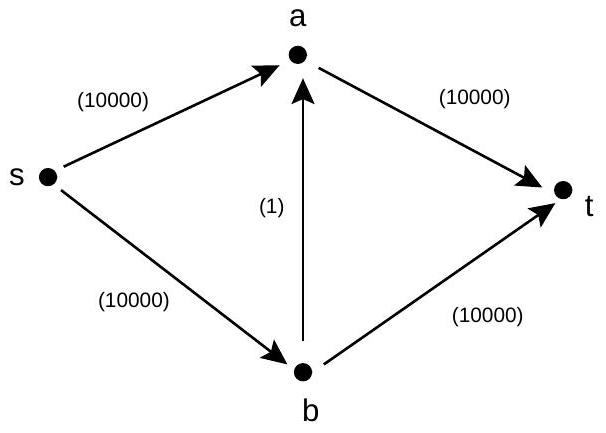
\includegraphics[max width=\textwidth, center]{2025_09_05_aa5f7b8425e7dd302062g-12(2)}

En este caso el valor del máximo flujo es 20000 . Veamos qué puede ocurrir cuando los caminos aumentativos no se eligen con una mínima cantidad de ramas. Partimos del flujo inicial $x=0$ y usamos el camino aumentativo $s \longrightarrow b \longrightarrow a \longrightarrow t$\\
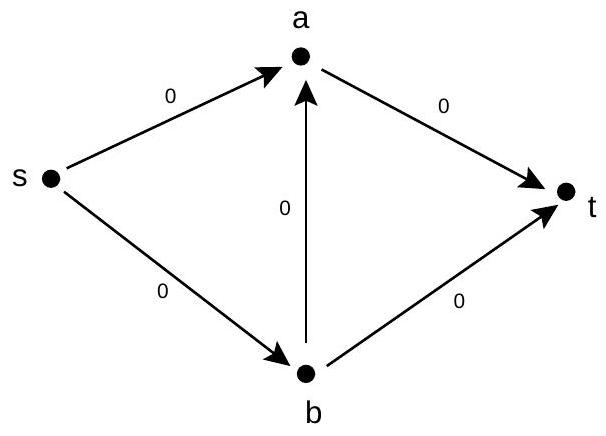
\includegraphics[max width=\textwidth, center]{2025_09_05_aa5f7b8425e7dd302062g-12}

En este camino todas las ramas son directas. Como la capacidad de la rama $(b, a)$ es 1 entonces $\delta=1$. Sumando $\delta=1$ al flujo de $(s, b),(b, a)$ y $(a, t)$ obtenemos el nuevo flujo\\
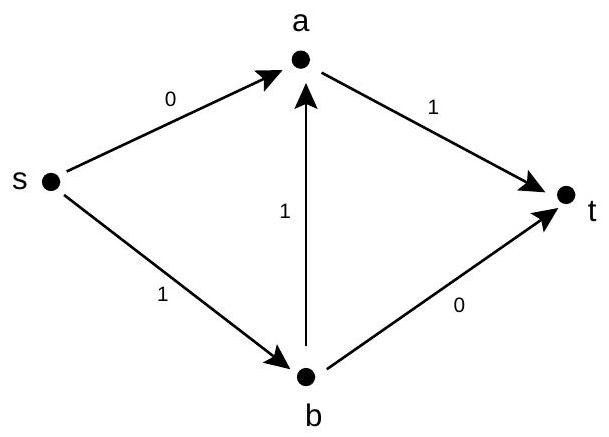
\includegraphics[max width=\textwidth, center]{2025_09_05_aa5f7b8425e7dd302062g-12(1)}

Ahora utilizamos el camino aumentativo $s \longrightarrow a \longleftarrow b \longrightarrow t$

En este camino las ramas $(s, a)$ y $(b, t)$ son directas y la rama $(b, a)$ es inversa. Como $x_{b a}=1$ entonces $\delta=1$. Sumando $\delta=1$ al flujo de las ramas $(s, a)$ y $(b, t)$ y restamos $\delta=1$ al flujo de la rama $(b, a)$, obtenemos\\
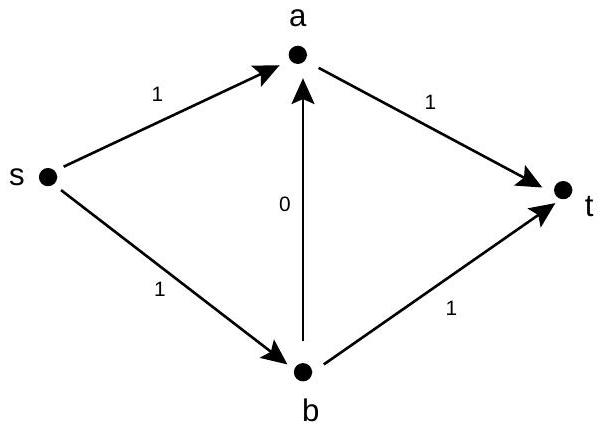
\includegraphics[max width=\textwidth, center]{2025_09_05_aa5f7b8425e7dd302062g-13(2)}

Como el flujo de la rama ( $b, a$ ) ahora es nulo entonces $s \longrightarrow b \longrightarrow a \longrightarrow t$ nuevamente es un camino aumentativo del presente flujo y $\delta=1$. Actualizando el flujo obtenemos\\
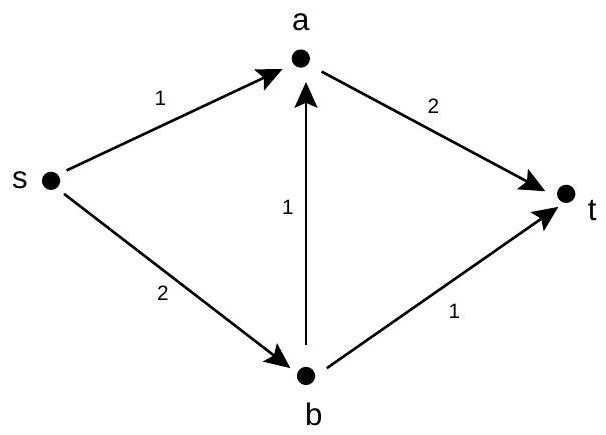
\includegraphics[max width=\textwidth, center]{2025_09_05_aa5f7b8425e7dd302062g-13}

Como $x_{b a}=1$, ahora $s \longrightarrow a \longleftarrow b \longrightarrow t$ es un camino aumentativo y $\delta=1$. Actualizando $x$ se tiene\\
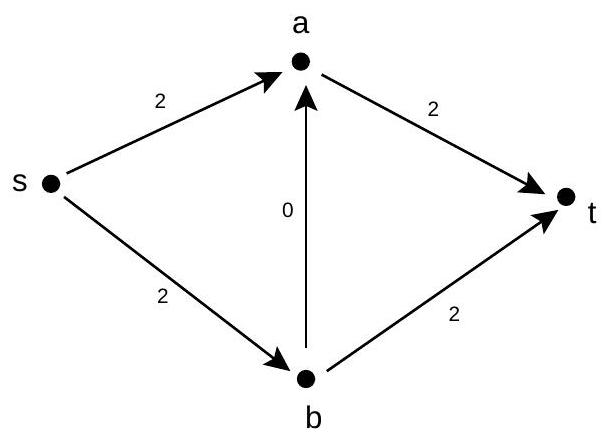
\includegraphics[max width=\textwidth, center]{2025_09_05_aa5f7b8425e7dd302062g-13(3)}

Es claro que si continuamos de esta manera necesitaremos 20000 iteraciones del algoritmo para llegar al óptimo. En cambio, si los caminos aumentativos son elegidos con un mínimo número de ramas, partiendo de $x=0$ primero usamos el camino aumentativo $s \longrightarrow a \longrightarrow t$ para aumentar el valor del flujo en $\delta=10000$ y obtenemos\\
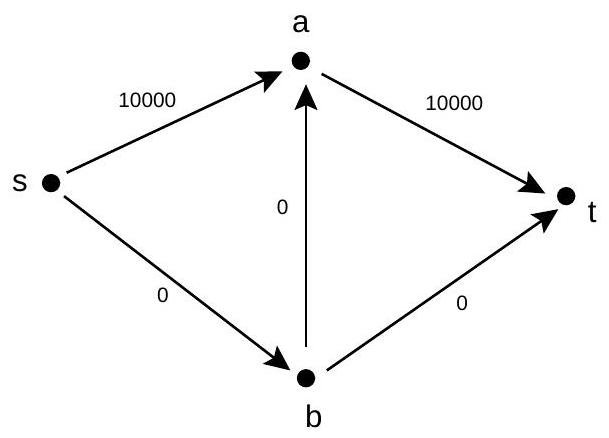
\includegraphics[max width=\textwidth, center]{2025_09_05_aa5f7b8425e7dd302062g-13(1)}\\
y luego usamos el camino aumentativo $s \longrightarrow b \longrightarrow t$ para aumentar nuevamente el valor del flujo en\\
$\delta=10000$, obtenemos en dos iteraciones el flujo óptimo\\
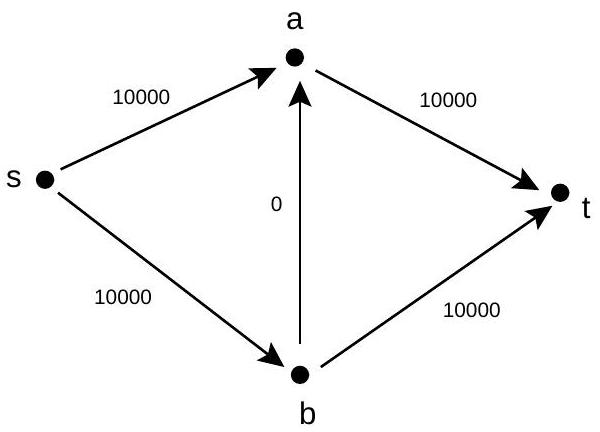
\includegraphics[max width=\textwidth, center]{2025_09_05_aa5f7b8425e7dd302062g-14(1)}

\section*{5. Aplicaciones.}
Veremos en esta sección una serie de aplicaciones tanto del problema de máximo flujo como del problema dual de hallar un mínimo corte.

\section*{a. Matching y cover.}
Definición 5.1. Sea $G=(V, E)$ un grafo. Diremos que un subconjunto $M$ de $E$ es un matching si no hay dos ramas de $M$ que incidan en un mismo vértice.

Definición 5.2. Sea $G=(V, E)$ un grafo. Diremos que un subconjunto $C$ de $V$ es un cover si, para cualquier rama en $E$, al menos uno de sus vértices pertenece a $C$.\\
Ejemplo 5.3. Dado el grafo\\
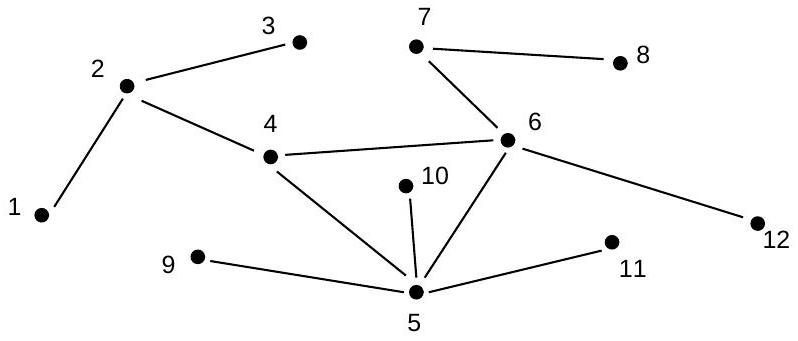
\includegraphics[max width=\textwidth, center]{2025_09_05_aa5f7b8425e7dd302062g-14}\\
los conjuntos $M_{1}=\{(2,4),(5,6),(7,8)\}$ y $M_{2}=\{(1,2),(4,6),(5,10),(7,8)\}$ son matchings y los conjuntos $C_{1}=\{2,5,6,8\}$ y $C_{2}=\{2,5,6,8,12\}$ son covers.\\
Lema 5.4. Sea $G=(V, E)$ un grafo. Si $M \subseteq E$ es un matching y $C \subseteq V$ es un cover entonces $\# M \leq \# C$.\\
Demostración: Sea $\varphi: M \longrightarrow C$ la aplicación definida por

$$
\varphi(u, v)= \begin{cases}u & \text { si } u \in C \\ v & \text { si } u \notin C\end{cases}
$$

Entonces valen\\
i) $\varphi$ está bien definida pues $C$ es un cover: si $u \notin C$ entonces $v \in C$.\\
ii) $\varphi$ es inyectiva pues $M$ es un matching.

Luego $\# M \leq \# C$. ㅁ\\
Definición 5.5 Sea $G=(V, E)$ un grafo. Diremos que $M \subseteq E$ es un máximo matching si $M$ es un matching y $\# M \geq \# M^{\prime}$ para todo matching $M^{\prime} \subseteq E$ y diremos que $C \subseteq V$ es un mínimo cover si $C$ es un cover y $\# C \leq \# C^{\prime}$ para todo cover $C^{\prime} \subseteq V$.

Observación 5.6. Dado un grafo $G$, si $M$ es un matching, $C$ es un cover y vale $\# M=\# C$ entonces, $M$ es un máximo matching y $C$ es un mínimo cover. En efecto, si $M^{\prime}$ es un matching entonces, por el lema 5.4., $\# M^{\prime} \leq \# C=\# M$ y análogamente, si $C^{\prime}$ es un cover, $\# C=\# M \leq \# C^{\prime}$.

\section*{Máximo matching y mínimo cover en un grafo bipartito.}
Sea $P$ un conjunto de hombres y sea $Q$ un conjunto de mujeres. Supongamos que para ciertos pares $(p, q) \in P \times Q p$ y $q$ se gustan mutuamente. Queremos hallar un número máximo de casamientos (suponiendo ingenuamente que para que dos personas se puedan casar deben gustarse mutuamente).

Representando esta situación en el grafo bipartito no dirigido $G=(V, E)$, donde $V=P \cup Q$ y donde $E=\{(p, q) \in P \times Q / p$ y $q$ se gustan mutuamente $\}$ (ver definición 1.9. del capítulo 2) el problema se traduce en hallar un máximo matching $M$ en el grafo bipartito $G$ (los elementos de $M$ serán los matrimonios formados).\\
Por ejemplo, consideremos el grafo bipartito\\
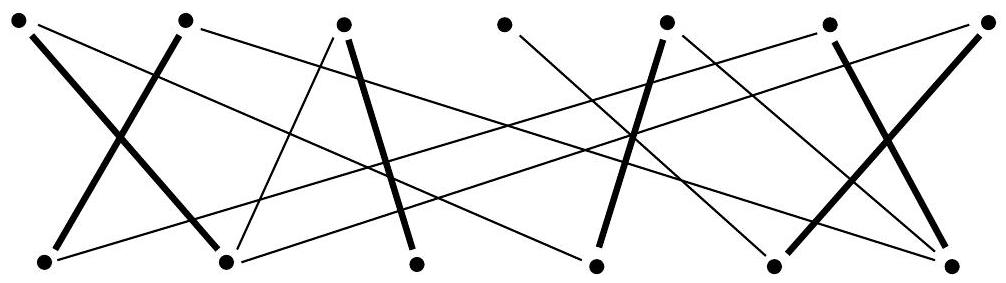
\includegraphics[max width=\textwidth, center]{2025_09_05_aa5f7b8425e7dd302062g-15(1)}

En este caso, el conjunto de las ramas indicadas con trazo grueso es un matching de cardinal seis.

Resolveremos el problema de hallar un máximo matching en $G$ como aplicación del problema de máximo flujo.\\
Construímos un nuevo grafo dirigido $G^{\prime}=\left(V^{\prime}, E^{\prime}\right)$ agregando a $G$ dos vértices $s$ y $t$ (que serán la fuente y la terminal respectivamente), ramas ( $s, p$ ) para cada $p \in P$ y ramas ( $q, t$ ) para cada $q \in Q$. A las ramas $(s, p)$ y ( $q, t$ ) les asignamos capacidad 1 y a las ramas ( $p, q$ ) dirección $p \longrightarrow q$ y capacidad infinita, es decir, $u_{s p}=1=u_{q t}$ y $u_{p q}=\infty(p \in P, q \in Q)$\\
En el ejemplo anterior el grafo $G^{\prime}$ sería\\
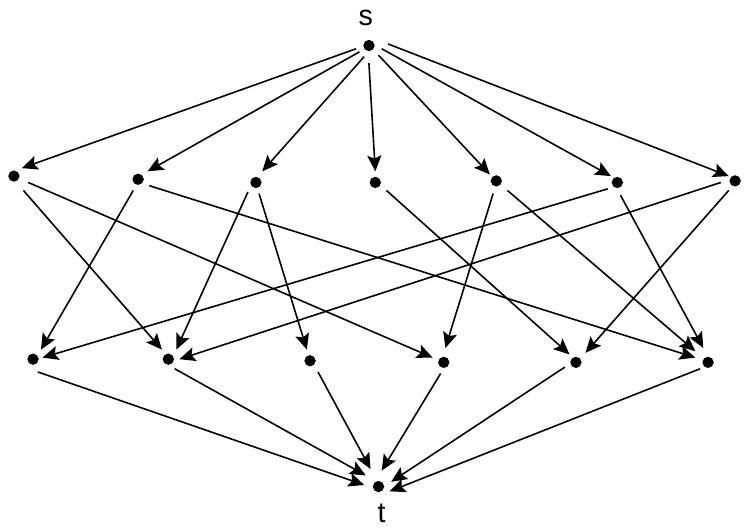
\includegraphics[max width=\textwidth, center]{2025_09_05_aa5f7b8425e7dd302062g-15}

Aplicamos el algoritmo de Ford-Fulkerson para hallar un máximo flujo entero $x$ de $G^{\prime}$ (ver observación 4.4.). Como $x$ es entero, por las capacidades definidas los valores de $x_{s p}$ y $x_{q t}$ sólo pueden ser cero o uno. Luego,\\
cada señor $p$ tendrá a lo sumo una pareja $q$ : como $x_{p q}$ es entero no negativo para todo $(p, q) \in E^{\prime}$ y

$$
x_{s p}=x(V, p)=x(p, V)=\sum_{\substack{q \in Q \\(p, q) \in E^{\prime}}} x_{p q}
$$

si $x_{s p}=0$ entonces $x_{p q}=0$ para todo $q$. En este caso el señor $p$ no integra ninguna feliz pareja. En cambio, si $x_{s p}=1$ entonces una y sólo una de las flechas ( $p, q$ ) tendrá flujo no nulo e igual a 1 . Esa es la señorita $q$ que le toca en suerte al señor $p$.\\
Recíprocamente, cada señorita $q$ tendrá a lo sumo una sola pareja $p$, ninguna cuando $x_{q t}=0$ y exactamente una cuando $x_{q t}=1$ ya que

$$
\sum_{\substack{p \in P \\(p, q) \in E^{\prime}}} x_{p q}=x(V, q)=x(q, V)=x_{q t}
$$

Esto muestra que $M=\left\{(p, q) \in E / x_{p q}=1\right\}$ es un matching de $G$. Notemos además que, como $x_{p q}=0$ o 1, entonces

$$
\# M=\sum_{p \in P} x(p, V)=\sum_{p \in P} x_{s p}=\text { valor de } x
$$

Sea $A$ el último conjunto generado por el algoritmo de Ford-Fulkerson antes de detenerse, es decir,

$$
A=\{s\} \cup\{v \in V / \exists \text { un camino aumentativo de } x \text { de } s \text { a } v\}
$$

Entonces $\partial A$ es un mínimo corte y su capacidad es igual al valor de $x$. Luego, la capacidad de $\partial A$ es finita y por lo tanto ninguna rama ( $p, q$ ) ( $p \in P, q \in Q$ ) pertenece a $\partial A$. Por otra parte, como $s \in A$ y $t \notin A$, si $p \in P$ y $q \in Q$ se tiene\\
i) $(s, p) \in \partial A$ sii $p \notin A$\\
ii) $(q, t) \in \partial A$ sii $q \in A$

Luego,

$$
\partial A=\{(s, p) / p \notin A\} \cup\{(q, t) / q \in A\}
$$

Como todas las ramas de $\partial A$ tienen capacidad 1 entonces se tiene que la capacidad del mínimo corte $\partial A$ es $\#(\partial A)=\#(P \cap \bar{A})+\#(Q \cap A)$.\\
Por otra parte, si $(p, q) \in E$ entonces $p \in P \cap \bar{A} \circ q \in Q \cap A$. En efecto, si $p \in P \cap A$ y $q \in Q \cap \bar{A}$ entonces $p \in A$ y $q \notin A$, de donde resultaría que $(p, q) \in \partial A$ cosa que vimos que no puede ocurrir. Esto muestra que el conjunto $C=(P \cap \bar{A}) \cup(Q \cap A)$ es un cover de $G$.\\
Luego, $\# C=\#(P \cap \bar{A})+\#(Q \cap A)=$ capacidad de $\partial A=$ valor de $x=\# M$. Por lo tanto, por la observación 5.6., resulta que $M$ es un máximo matching, $C$ es un mínimo cover y $\# M=\# C$.

Notemos que no sólo encontramos un máximo matching $M$ de $G$ sino que también hallamos un mínimo cover del mismo cardinal. Es decir, al mismo tiempo que resolvimos el problema de los matrimonios hemos demostrado el siguiente

Teorema 5.7. (König) En un grafo bipartito no dirigido el cardinal de un máximo matching es igual al cardinal de un mínimo cover.

\section*{b. Cierre óptimo en un grafo dirigido.}
Supongamos que tenemos $m$ proyectos y que cada proyecto $v$ tiene asignado un número entero $b_{v}$ que llamaremos beneficio (pero que podría ser negativo a pesar de llamarse beneficio). Supongamos además que hay ciertos proyectos que requieren de la realización de otros. Queremos encontrar un subconjunto $A$ de\\
proyectos tal que si $u \in A$ entonces $v \in A$ para todo proyecto $v$ que se requiera para realizar $u$ y de manera que $\sum_{v \in A} b_{v}$ sea máximo.\\
Sea $G=(V, E)$ el grafo dirigido cuyos vértices son los proyectos y cuyas ramas son los pares ( $u, v$ ) tales que $v$ se requiere para realizar $u$. Entonces, hallar un subconjunto $A$ de proyectos que satisfaga

$$
u \in A \quad \Longrightarrow \quad v \in A \quad \forall v \text { que se requiera para realizar } u
$$

es lo mismo que hallar un subconjunto $A$ de $V$ tal que el corte definido por $A$ en $G$ sea vacío.\\
Definición 5.8. Dado un grafo $G=(V, E)$ diremos que un subconjunto $A$ de $V$ es cerrado si $\partial A=\emptyset$. Si, además, cada $v \in V$ tiene asignado un número real $b_{v}$ diremos que $A \subseteq V$ es un cierre óptimo en $G$ si $A$ es cerrado y $\sum_{v \in A} b_{v} \geq \sum_{v \in A^{\prime}} b_{v}$ para todo subconjunto cerrado $A^{\prime}$ de $V$.\\
De esta manera nuestro problema se traduce en encontrar un cierre óptimo en $G$. Por ejemplo, si $b_{v} \geq 0$ para todo $v \in V$ entonces basta tomar $A=V$ y si $b_{v} \leq 0$ para todo $v \in V$ entonces basta tomar $A=\emptyset$.\\
Para resolver este problema construímos, a partir de $G$, un nuevo grafo $G^{\prime}$ agregando dos vértices $s$ y $t$ (la fuente y la terminal), ramas ( $s, v$ ) para cada $v$ tal que $b_{v}>0$ con capacidad $b_{v}$ y ramas ( $v, t$ ) para cada $v$ tal que $b_{v}<0$ con capacidad $-b_{v}$. A las ramas de $E$ les asignamos capacidad infinita.\\
Sea $\partial B$ un mínimo corte en $G^{\prime}$ (tal que $s \in B$ y $t \notin B$ ). Como la capacidad de $\partial B$ es menor o igual que la capacidad del corte definido por $\{s\}$ en $G^{\prime}$ y todas las ramas de $G^{\prime}$ que salen de $s$ tienen capacidad finita, entonces $\partial B$ es un corte de capacidad finita. Luego, ninguna rama de $E$ puede pertenecer a $\partial B$ ya que esas ramas tienen capacidad infinita.\\
Sea $A$ el subconjunto de $V$ definido por $A=B-\{s\}$. Como el corte definido por $B$ en $G^{\prime}$ no contiene ninguna rama de $E$ entonces el corte definido por $A$ en $G$ no contiene ninguna rama de $E$, es decir, es vacío. Esto muestra que $A$ es un subconjunto cerrado de $V$. Además, $(s, v) \in \partial B$ sii $b_{v}>0$ y $v \notin A$ y $(v, t) \in \partial B$ sii $b_{v}<0$ y $v \in A$. Luego, la capacidad del corte es

$$
\begin{aligned}
& \sum_{\substack{v \notin A \\
b_{v}>0}} b_{v}-\sum_{\substack{v \in A \\
b_{v}<0}} b_{v}= \\
= & \sum_{\substack{v \notin A \\
b_{v} \geq 0}} b_{v}+\sum_{\substack{v \in A \\
b_{v} \geq 0}} b_{v}-\sum_{\substack{v \in A \\
b_{v} \geq 0}} b_{v}-\sum_{\substack{v \in A \\
b_{v}<0}} b_{v}= \\
= & \sum_{\substack{v \in V \\
b_{v} \geq 0}} b_{v}-\sum_{v \in A} b_{v}
\end{aligned}
$$

Supongamos ahora que $A^{\prime}$ es un subconjunto cerrado de $V$. Consideremos el corte definido por $B^{\prime}=A^{\prime} \cup\{s\}$ en $G^{\prime}$. Entonces $\partial B^{\prime}$ no contiene ninguna rama de $E$ (pues $A^{\prime}$ es cerrado) y, además, $(s, v) \in \partial B^{\prime}$ sii $b_{v}>0$ y $v \notin A^{\prime}$ y $(v, t) \in \partial B^{\prime}$ sii $b_{v}<0$ y $v \in A^{\prime}$. Luego, la capacidad de $\partial B^{\prime}$ es

$$
\begin{aligned}
& \sum_{\substack{v \notin A^{\prime} \\
b_{v}>0}} b_{v}-\sum_{\substack{v \in A^{\prime} \\
b_{v}<0}} b_{v}= \\
= & \sum_{\substack{v \notin A^{\prime} \\
b_{v} \geq 0}} b_{v}+\sum_{\substack{v \in A^{\prime} \\
b_{v} \geq 0}} b_{v}-\sum_{\substack{v \in A^{\prime} \\
b_{v} \geq 0}} b_{v}-\sum_{\substack{v \in A^{\prime} \\
b_{v}<0}} b_{v}= \\
= & \sum_{\substack{v \in V \\
b_{v} \geq 0}} b_{v}-\sum_{v \in A^{\prime}} b_{v}
\end{aligned}
$$

Dado que $\partial B$ era un mínimo corte en $G^{\prime}$ entonces su capacidad debe ser menor o igual que la de $\partial B^{\prime}$ de donde

$$
\sum_{v \in A} b_{v}=\sum_{\substack{v \in V \\ b_{v} \geq 0}} b_{v}-\text { capacidad de } \partial B \geq \sum_{\substack{v \in V \\ b_{v} \geq 0}} b_{v}-\text { capacidad de } \partial B^{\prime}=\sum_{v \in A^{\prime}} b_{v}
$$

y por lo tanto resulta que $A$ es un cierre óptimo en $G$.

\section*{c. Eligiendo localidades.}
Sea $G=(V, E)$ un grafo no dirigido. Supongamos que la elección del vértice $u$ implica un costo $c_{u}>0 (u \in V)$ y que la elección de una rama ( $u, v$ ) implica un beneficio $b_{u v}>0((u, v) \in E)$. Queremos elegir un subconjunto $S$ de $V$ tal que el beneficio neto asociado a esa elección definido por

$$
\sum_{\substack{(u, v) \in E \\ u \in S, v \in S}} b_{u v}-\sum_{u \in S} c_{u}
$$

sea máximo.\\
Para resolver este problema creamos un nuevo grafo dirigido $G^{\prime}=\left(V^{\prime}, E^{\prime}\right)$ poniendo, para cada vértice $u$ de $G$, un vértice $u$ en $G^{\prime}$ y, para cada rama ( $u, v$ ) de $G$, un único vértice $u v$ en $G^{\prime}$. Ahora agregamos dos vértices más: la fuente $s$ y la terminal $t$. Además, para cada vértice $u v$ de $G^{\prime}$ ponemos una rama dirigida $(s, u v)$ con capacidad $b_{u v}$ y dos ramas dirigidas $(u v, u)$ y $(u v, v)$ con capacidad infinita. Finalmente, para cada vértice $u$ de $G^{\prime}$ ponemos una rama dirigida $(u, t)$ con capacidad $c_{u}$. Por ejemplo, si $G$ es el grafo no dirigido\\
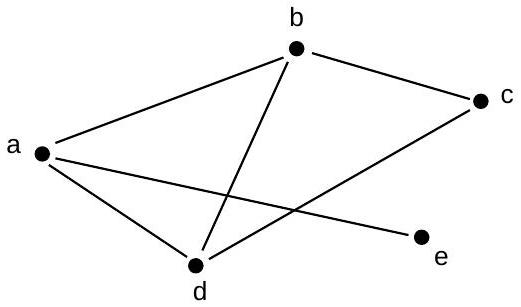
\includegraphics[max width=\textwidth, center]{2025_09_05_aa5f7b8425e7dd302062g-18}\\
entonces $G^{\prime}$ será el grafo dirigido\\
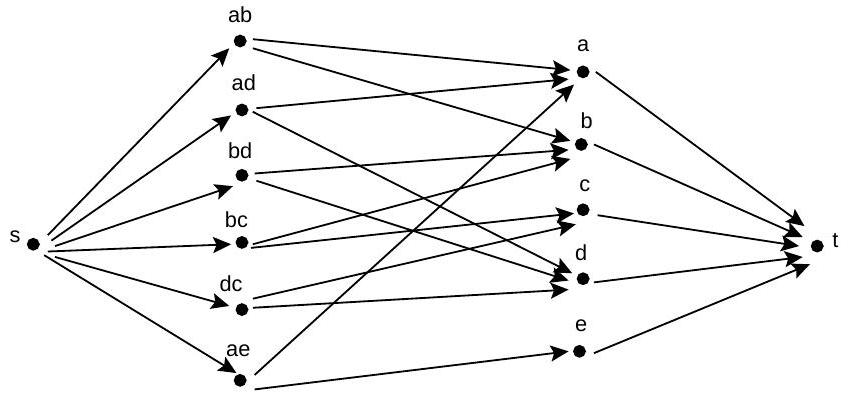
\includegraphics[max width=\textwidth, center]{2025_09_05_aa5f7b8425e7dd302062g-18(1)}

Observación 5.9. Sea $A \subseteq V^{\prime}$ tal que $s \in A$ y $t \notin A$. Entonces $(s, u v) \in \partial A$ sii $u v \notin A$ (donde $u v$ es el vértice de $G^{\prime}$ correspondiente a la rama $(u, v)$ de $G$ ) y $(u, t) \in \partial A$ sii $u \in V \cap A$. Si además el corte $\partial A$ tiene capacidad finita entonces ninguna rama ( $u v, u$ ) o ( $u v, v$ ) pertenece al corte.\\
Luego, si $\partial A$ es un corte de capacidad finita entonces

$$
\text { capacidad de } \partial A=\sum_{\substack{u v \in V^{\prime} / \\ u v \notin A}} b_{u v}+\sum_{u \in V \cap A} c_{u}
$$

Observación 5.10. Sea $A \subseteq V^{\prime}$ tal que $s \in A, t \notin A, \partial A$ tiene capacidad finita y tal que para todo $u, v$ se verifica

$$
u v \in A \Longleftrightarrow u \in A \cap V, v \in A \cap V \text { y }(u, v) \in E
$$

Entonces

$$
\begin{aligned}
& \sum_{u v \in V^{\prime}} b_{u v}-\text { capacidad de } \partial A= \\
= & \sum_{u v \in V^{\prime}} b_{u v}-\sum_{u v \notin A} b_{u v}-\sum_{u \in A \cap V} c_{u}= \\
= & \sum_{u v \in A} b_{u v}-\sum_{u \in A \cap V} c_{u}= \\
= & \sum_{\substack{(u, v) \in E / \\
u \in A \cap V, v \in A \cap V}} b_{u v}-\sum_{u \in A \cap V} c_{u}
\end{aligned}
$$

Sea ahora $x$ un flujo en $G^{\prime}$ de valor máximo y sea $\partial A$ el correspondiente mínimo corte. Entonces la capacidad de $\partial A$ es finita ya que es menor o igual que la capacidad del corte definido por $\{s\}$. Veamos que $A$ verifica $u v \in A$ sii $u \in A \cap V, v \in A \cap V$ y $(u, v) \in E$ :\\
Sea $u v \in V^{\prime}$. Si $u v \in A$, como $\partial A$ es de capacidad finita entonces $(u v, u) \notin \partial A$ y $(u v, v) \notin \partial A$. Luego, $u \in A \cap V$ y $v \in A \cap V$. Además, $(u, v) \in E$ pues $u v \in V^{\prime}$.\\
Recíprocamente, si $u \in A \cap V, v \in A \cap V$ y $(u, v) \in E$ entonces $u v \in V^{\prime}$. Como el valor de $x$ es igual a la capacidad de $\partial A$, por la observación 4.5. se tiene

$$
x_{e}=u_{e} \forall e \in \partial A \text { y } x_{e}=0 \forall e \in \partial \bar{A}
$$

Supongamos que $u v \notin A$. En tal caso $(s, u v) \in \partial A$ y $(u v, u),(u v, v) \in \partial \bar{A}$, de donde $x_{s u v}=b_{u v}>0$ y $x_{u v u}=0=x_{u v v}$.\\
Entonces $0=x_{u v u}+x_{u v v}=x\left(u v, V^{\prime}\right)=x\left(V^{\prime}, u v\right)=x_{s u v}=b_{u v}$. Absurdo, pues $b_{u v}>0$. Luego $u v \in A$.\\
Por lo tanto, $\partial A$ es un corte de capacidad finita y verifica $u v \in A$ sii $u \in A \cap V$ y $v \in A \cap V$. Luego, por la observación 5.10 vale

$$
\begin{aligned}
& \sum_{u v \in V^{\prime}} b_{u v}-\text { capacidad de } \partial A= \\
= & \sum_{\substack{(u, v) \in E / \\
u \in A \cap V, v \in A \cap V}} b_{u v}-\sum_{u \in A \cap V} c_{u}
\end{aligned}
$$

Por lo tanto, tomando $S=A \cap V$ se tiene que

$$
\begin{aligned}
& \sum_{u v \in V^{\prime}} b_{u v}-\text { capacidad de } \partial A= \\
= & \sum_{\substack{(u, v) \in E / \\
u \in S, v \in S}} b_{u v}-\sum_{u \in S} c_{u}
\end{aligned}
$$

Si $S^{\prime}$ es un subconjunto de $V$ entonces $B=S^{\prime} \cup\{s\} \cup\left\{u v \in V^{\prime} / u \in S^{\prime}\right.$ y $\left.v \in S^{\prime}\right\}$ es un subconjunto de $V^{\prime}$ que contiene a $s$ y no a $t$. Luego la capacidad del corte definido por $A$ en $G^{\prime}$ debe ser menor o igual que la capacidad de $\partial B$.\\
Veamos cuáles ramas pertenecen a $\partial B$. Como $s \in B$ entonces $(s, u v) \in \partial B$ sii $u v \notin B$ y como $t \notin B$ entonces $(u, t) \in \partial B$ sii $u \in V \cap B$. Además, ninguna rama $(u v, u)$ o $(u v, v)$ pertenece a $\partial B$ pues si $u v \in B$ entonces $u \in S^{\prime}$ y $v \in S^{\prime}$ y por lo tanto $u \in B$ y $v \in B$. Luego la capacidad del corte $\partial B$ es finita. Más aún, $B$ satisface

$$
u v \in B \quad \Longleftrightarrow \quad u \in B \cap V, v \in B \cap V \mathrm{y}(u, v) \in E
$$

y, teniendo en cuenta que $V \cap B=S^{\prime}$, por la observación 5.10. resulta que

$$
\begin{aligned}
& \sum_{u v \in V^{\prime}} b_{u v}-\text { capacidad de } \partial B= \\
& \sum_{\substack{(u, v) \in E / \\
u \in B \cap V, v \in B \cap V}} b_{u v}-\sum_{u \in B \cap V} c_{u}= \\
= & \sum_{\substack{(u, v) \in E / \\
u \in S^{\prime}, v \in S^{\prime}}} b_{u v}-\sum_{u \in S^{\prime}} c_{u}
\end{aligned}
$$

Como capacidad de $\partial A \leq$ capacidad de $\partial B$ entonces

$$
\begin{aligned}
& \sum_{\substack{(u, v) \in E / \\
u \in S, v \in S}} b_{u v}-\sum_{u \in S} c_{u}=\sum_{u v \in V^{\prime}} b_{u v}-\text { capacidad de } \partial A \geq \\
\geq & \sum_{u v \in V^{\prime}} b_{u v}-\text { capacidad de } \partial B=\sum_{\substack{(u, v) \in E / \\
u \in S^{\prime}, v \in S^{\prime}}} b_{u v}-\sum_{u \in S^{\prime}} c_{u}
\end{aligned}
$$

Hemos probado entonces que si $S^{\prime}$ es cualquier subconjunto de $V$ entonces

$$
\sum_{\substack{(u, v) \in E / \\ u \in S, v \in S}} b_{u v}-\sum_{u \in S} c_{u} \geq \sum_{\substack{(u, v) \in E / \\ u \in S^{\prime}, v \in S^{\prime}}} b_{u v}-\sum_{u \in S^{\prime}} c_{u}
$$

Luego, si $\partial A$ es el mínimo corte correspondiente a un máximo flujo $x$ en $G^{\prime}$, entonces $S=A \cap V$ es el subconjunto de $V$ que satisface

$$
\sum_{\substack{(u, v) \in E \\ u \in S, v \in S}} b_{u v}-\sum_{u \in S} c_{u}
$$

es máximo.

\section*{d. Asignación de tareas.}
Supongamos que se desea realizar $m$ tareas en $n$ días. Sea $p_{u}$ el número de horas necesarias para realizar la tarea $u(1 \leq u \leq m)$ y sea $q_{v}$ el número de horas disponibles en el día $v(1 \leq v \leq n)$. Supongamos además que cada tarea $u$ no puede iniciarse antes del día $s_{u}$ ni terminarse después del día $t_{u}$. Las tareas no necesariamente deben realizarse en un mismo día, pero una parte de la tarea $u$ (que podría ser toda) puede asignarse al día $v$ sii $s_{u} \leq v \leq t_{u}$. El problema consiste en determinar si la asignación de tareas es factible y, en tal caso, hallar una solución factible del problema.\\
Representaremos la situación en un grafo dirigido bipartito $G=(V, E)$ donde $V=\{$ tareas $\} \cup\{$ días $\}$ y haya una rama ( $u, v$ ) cuando parte de la tarea $u$ puede asignarse al día $v$ (es decir, cuando $s_{u} \leq v \leq t_{u}$ ). Sea $x_{u v}$ la cantidad de horas del día $v$ que se dedicarían a la realización de una parte (que podría ser toda) de la tarea $u$. Entonces la asignación de tareas es factible sii existe $x$ tal que


\begin{align*}
& \sum_{v} x_{u v}=p_{u} \quad \forall u \\
& \sum_{u} x_{u v} \leq q_{v} \quad \forall v  \tag{1}\\
& x_{u v} \geq 0 \quad \forall(u, v) \in E
\end{align*}


Para averiguar si existe una solución factible creamos un nuevo grafo dirigido $G^{\prime}$ agregando al grafo $G$ dos vértices $s$ y $t$, para cada tarea $u$ una rama $(s, u)$ con capacidad $p_{u}$ y para cada día $v$ una rama $(v, t)$ con capacidad $q_{v}$. A las ramas de $(u, v) \in E$ les asignamos capacidad infinita.

Proposición 5.11. El problema de asignación de tareas es factible si y sólo si $G^{\prime}$ tiene un flujo $x$ de valor máximo que satisface $x_{s u}=p_{u}$ para toda tarea $u$. En tal caso, ( $x_{u v}$ ) es una solución factible de (1).\\
Demostración: Si el problema es factible y $x_{u v}$ es una solución de (1) tomando $x_{s u}=p_{u}$ y $x_{v t}=\sum_{u} x_{u v}$ se tiene que $x$ es un flujo factible en $G^{\prime}$, es decir es un b-flujo (pues $x(u, V)=\sum_{v} x_{u v}=p_{u}=x_{s u}=x(V, u)$ para toda tarea $u$ y, para todo día $\left.v, x(V, v)=\sum_{u} x_{u v}=x_{v t}=x(v, V)\right)$ y para toda rama $e$ de $G^{\prime}, x_{e}$ es no negativo y menor o igual que la capacidad de la rama (pues $x_{s u}=p_{u}$ y $x_{v t}=\sum_{u} x_{u v} \leq q_{v}$ ).\\
Además, como no existe un camino aumentativo de $x$ de $s$ a $t$ pues para cada tarea $u$ vale $x_{s u}=p_{u}=$ capacidad de la rama $(s, u)$ entonces el valor de este flujo debe ser máximo.\\
Recíprocamente, si $x$ es un flujo de valor máximo que satisface $x_{s u}=p_{u}$ para toda tarea $u$ entonces $x_{u v} \geq 0$,

$$
\sum_{v} x_{u v}=x(u, V)=x(V, u)=x_{s u}=p_{u}
$$

y

$$
\sum_{u} x_{u v}=x(V, v)=x(v, V)=x_{v t} \leq q_{v}
$$

pues $q_{v}$ es la capacidad de la rama ( $v, t$ ), es decir, ( $x_{u v}$ ) es solución de (1). ㅁ\\
Corolario 5.12. El problema de asignación de tareas es factible si y sólo si $G^{\prime}$ tiene un flujo máximo de valor $\sum_{u} p_{u}$.\\
Demostración: Si el problema de asignación es factible entonces $G^{\prime}$ tiene un flujo $x$ de valor máximo que satisface $x_{s u}=p_{u}$ para toda tarea $u$. Por lo tanto el valor de $x$ es igual a $\sum_{u} x_{s u}=\sum_{u} p_{u}$. Recíprocamente, sea $x$ un flujo óptimo en $G^{\prime}$ de valor $\sum_{u} p_{u}$.\\
Como $x_{s u} \leq$ capacidad de la rama $(s, u)=p_{u}$ y como $\sum_{u} x_{s u}=$ valor de $x=\sum_{u} p_{u}$ entonces debe ser $x_{s u}=p_{u}$ para toda tarea $u$ (pues si para algún $u$ fuese $x_{s u}<p_{u}$ entonces resultaría que $\sum x_{s u}<\sum p_{u}$ ). ㅁ

\section*{e. El problema del transshipment.}
Sea $G=(V, E)$ un grafo dirigido donde cada vértice $v \in V$ tiene asignado un número real $b_{v}$ y cada rama $e \in E$ tiene asignada una capacidad $u_{e}$ tal que $0<u_{e} \leq \infty$.\\
Queremos determinar si existe $x=\left(x_{e}\right)_{e \in E}$ que satisfaga

$$
\begin{aligned}
x(v, V)-x(V, v)=b_{v} & \forall v \in V \\
0 \leq x_{e} \leq u_{e} & (e \in E)
\end{aligned}
$$

Este problema se conoce como el problema del transshipment.\\
Observemos que

$$
\begin{aligned}
& \sum_{v} x(v, V)-x(V, v)= \\
= & \sum_{v}\left(\sum_{w /(v, w) \in E} x_{v w}-\sum_{w /(w, v) \in E} x_{w v}\right)= \\
= & \sum_{e \in E} x_{e}-\sum_{e \in E} x_{e}=0
\end{aligned}
$$

y, por lo tanto, una condición necesaria para que el problema sea factible (es decir, para que exista $x$ ) es que valga

$$
\sum_{v \in V} b_{v}=0
$$

Para resolver este problema creamos, a partir del grafo $G=(V, E)$, un nuevo grafo dirigido $G^{\prime}$ de la siguiente manera: agregamos a $V$ dos vértices $s$ y $t$ (que serán la fuente y la terminal), para cada $v$ tal que $b_{v}>0$ agregamos una rama ( $s, v$ ) con capacidad $b_{v}$ y, para cada $v$ tal que $b_{v}<0$ agregamos una rama ( $v, t$ ) con capacidad $-b_{v}$. A las ramas de $e \in E$ les asignamos capacidad $u_{e}$.

Proposición 5.13. El problema del transshipment es factible sii $G^{\prime}$ tiene un flujo máximo $x$ que verifica

$$
\begin{aligned}
& x_{s u}=b_{u} \quad \forall u / b_{u}>0 \\
& x_{u t}=-b_{u} \quad \forall u / b_{u}<0
\end{aligned}
$$

Demostración: $G^{\prime}=\left(V^{\prime}, E^{\prime}\right)$, donde

$$
V^{\prime}=V \cup\{s, t\}
$$

y

$$
E^{\prime}=E \cup\left\{(s, u) / b_{u}>0\right\} \cup\left\{(u, t) / b_{u}<0\right\}
$$

$(\Longleftarrow)$ Sea $\left(x_{e}\right)_{e \in E^{\prime}}$ un flujo máximo en $G^{\prime}$ que verifica

$$
\begin{aligned}
& x_{s u}=b_{u} \quad \forall u / b_{u}>0 \\
& x_{u t}=-b_{u} \quad \forall u / b_{u}<0
\end{aligned}
$$

Luego, $0 \leq x_{e} \leq u_{e}$ para todo $e \in E$. Sea $u \neq s$,t.\\
Si $b_{u}>0$ entonces

$$
\begin{aligned}
& x(u, V)-x(V, u)=\sum_{v /(u, v) \in E} x_{u v}-\sum_{v /(v, u) \in E} x_{v u}= \\
= & x\left(u, V^{\prime}\right)-x\left(V^{\prime}, u\right)+x_{s u}=x_{s u}=b_{u}
\end{aligned}
$$

y, si $b_{u}<0$ entonces

$$
\begin{aligned}
& x(u, V)-x(V, u)=\sum_{v /(u, v) \in E} x_{u v}-\sum_{v /(v, u) \in E} x_{v u}= \\
= & x\left(u, V^{\prime}\right)-x\left(V^{\prime}, u\right)-x_{u t}=-x_{u t}=b_{u}
\end{aligned}
$$

Luego, $\left(x_{e}\right)_{e \in E}$ es una solución del problema del transshipment.\\
$(\Longrightarrow)$ Sea $\left(x_{e}\right)_{e \in E}$ una solución del problema. Tomando

$$
\begin{aligned}
& x_{s u}=b_{u} \quad \forall u / b_{u}>0 \\
& x_{u t}=-b_{u} \quad \forall u / b_{u}<0
\end{aligned}
$$

resulta que $\left(x_{e}\right)_{e \in E^{\prime}}$ es un flujo máximo de $G^{\prime}$. En efecto, para toda rama $e \in E^{\prime} x_{e}$ es no negativo y no excede la capacidad de la rama. Además, es un b-flujo: para todo $u \in V^{\prime}, u \neq s, t$ es

$$
x\left(u, V^{\prime}\right)-x\left(V^{\prime}, u\right)=\left\{\begin{array}{ll}
x(u, V)-x(V, u)-x_{s u} & \text { si } b_{u}>0 \\
x(u, V)-x(V, u)-x_{u t} & \text { si } b_{u}<0
\end{array}=\left\{\begin{array}{ll}
b_{u}-x_{s u} & \text { si } b_{u}>0 \\
b_{u}+x_{u t} & \text { si } b_{u}<0
\end{array}=0\right.\right.
$$

Por último, $x$ es de valor máximo ya que para las ramas que salen de $s$ se tiene $x_{s u}=b_{u}=$ capacidad de la rama $(s, u)$.

Corolario 5.14. El problema del transshipment es factible si y sólo si $G^{\prime}$ tiene un flujo máximo de valor $\sum_{u / b_{u}>0} b_{u}$ У $\sum_{u} b_{u}=0$.\\
Dejamos la demostración como tarea para el lector.\\
Observación 5.15. Notar que hallando un máximo flujo $x$ en $G^{\prime}$ no sólo podemos determinar si el problema del transshipment es factible sino que, cuando lo es, podemos hallar una solución.\\
En efecto, sea $x=\left(x_{e}\right)_{e \in E^{\prime}}$ un máximo flujo en $G^{\prime}$ y supongamos que $\sum_{u} b_{u}=0$ y valor de $x=\sum_{u / b_{u}>0} b_{u}$ (si alguna de estas condiciones no valiera sabemos que el problema del transshipment no es factible).\\
Como valor de $x=\sum_{u / b_{u}>0} b_{u}$ entonces necesariamente se tiene que $x_{s u}=b_{u} \quad \forall u / b_{u}>0$ pues

$$
x_{s u} \leq b_{u} \quad \forall u / b_{u}>0 \text { y } \sum_{u / b_{u}>0} x_{s u}=\sum_{(s, u) \in E^{\prime}} x_{s u}=\text { valor de } x=\sum_{u / b_{u}>0} b_{u}
$$

Además, como $\sum_{u} b_{u}=0$ entonces $\sum_{u / b_{u}>0} b_{u}=-\sum_{u / b_{u}<0} b_{u}$ de donde resulta que $x_{u t}=-b_{u} \quad \forall u / b_{u}<0$ pues $x_{u t} \leq-b_{u} \quad \forall u / b_{u}<0 \mathrm{y}$

$$
\begin{aligned}
& \sum_{u / b_{u}<0} x_{u t}=\sum_{(u, t) \in E^{\prime}} x_{u t}=x\left(V^{\prime}, t\right)-x\left(t, V^{\prime}\right)= \\
& \quad=x\left(s, V^{\prime}\right)-x\left(V^{\prime}, s\right)=\text { valor de } x=\sum_{u / b_{u}>0} b_{u}=-\sum_{u / b_{u}<0} b_{u}=\sum_{u / b_{u}<0}\left(-b_{u}\right)
\end{aligned}
$$

Luego $\left(x_{e}\right)_{e \in E^{\prime}}$ un flujo máximo en $G^{\prime}$ que verifica

$$
\begin{aligned}
& x_{s u}=b_{u} \quad \forall u / b_{u}>0 \\
& x_{u t}=-b_{u} \quad \forall u / b_{u}<0
\end{aligned}
$$

y por lo tanto se tiene que $\left(x_{e}\right)_{e \in E}$ es una solución al problema del transshipment (ver demostración de la proposición 5.13.).

\section*{f. El problema del torneo.}
En un torneo hay $n$ equipos que juegan todos contra todos, exactamente una vez. Supongamos que el resultado de un encuentro no puede ser un empate.\\
Dado un vector $\alpha=\left(\alpha_{1}, \ldots, \alpha_{n}\right) \in \mathbb{N}^{n}$ diremos que $\alpha$ es factible si existe una asignación de resultados a los partidos tal que, para cada $i, \alpha_{i}$ sea la cantidad de partidos ganados por el equipo $i$ al terminar el torneo. El problema consiste en determinar si un dado un vector $\left(\alpha_{1}, \ldots, \alpha_{n}\right)$ es factible.\\
Para resolverlo, construímos un grafo dirigido $G=(V, E)$, donde $V=\{1,2, \ldots, n\}$ y $E=\{(u, v) / u<v\}$. A cada rama ( $u, v$ ) le asignamos capacidad 1.\\
Para cada $u<v$ sea $x_{u v}$ el número de partidos que el equipo $u$ le ganó al equipo $v$ en el torneo. Como cada par de equipos se enfrenta una y sólo una vez entonces debe ser $x_{u v}=0$ o $x_{u v}=1$, es decir, $0 \leq x_{u v} \leq 1$ y $x_{u v}$ entero.\\
Sean $u, v \in V, u \neq v$. Si $u<v$ entonces $u$ le ganó a $v$ si y sólo si $x_{u v}=1$ y si $v<u$ entonces $u$ le ganó a $v$ si y sólo si $v$ perdió con $u$ sii $x_{v u}=0$ sii $1-x_{v u}=1$. Luego, el número de partidos que $u$ ganó jugando contra los equipos $u+1, u+2, \ldots, n$ es

$$
\sum_{v /(u, v) \in E} x_{u v}
$$

y el número de partidos que $u$ ganó jugando contra los equipos $1,2, \ldots, u-1$ es

$$
\sum_{v /(v, u) \in E}\left(1-x_{v u}\right)=(u-1)-\sum_{v /(v, u) \in E} x_{v u}
$$

Luego, $\left(\alpha_{1}, \ldots, \alpha_{n}\right)$ es factible sii existe $x=\left(x_{u v}\right)_{(u, v) \in E}$ entero tal que $0 \leq x_{u v} \leq 1 \mathrm{y}$

$$
\sum_{v /(u, v) \in E} x_{u v}+(u-1)-\sum_{v /(v, u) \in E} x_{v u}=\alpha_{u}
$$

es decir, tal que

$$
\begin{gathered}
x(u, V)-x(V, u)=\alpha_{u}+(1-u) \quad \forall u \in V \\
0 \leq x_{e} \leq 1 \quad(e \in E)
\end{gathered}
$$

De esta forma, hemos planteado el problema del torneo como un problema de transshipment en el cual $b_{u}=\alpha_{u}+(1-u)$.\\
Observemos que, como se juegan $\binom{n}{2}$ partidos, entonces una condición necesaria para que $\left(\alpha_{1}, \ldots, \alpha_{n}\right)$ sea factible es que

$$
\sum_{u} \alpha_{u}=\binom{n}{2}
$$

Esta condición es equivalente a $\sum_{u} b_{u}=0$, que es la condición necesaria para que el problema, visto como un problema de transshipment, sea factible.\\
En efecto,

$$
\begin{aligned}
& \sum_{u} b_{u}=0 \text { sii } \sum_{u=1}^{n}\left(\alpha_{u}+1-u\right)=0 \text { sii } \\
& \text { sii } \sum_{u=1}^{n} \alpha_{u}+\sum_{u=1}^{n}(1-u)=0 \text { sii } \sum_{u=1}^{n} \alpha_{u}=\sum_{u=1}^{n}(u-1) \text { sii } \\
& \text { sii } \sum_{u=1}^{n} \alpha_{u}=\frac{n(n-1)}{2} \text { sii } \sum_{u=1}^{n} \alpha_{u}=\binom{n}{2}
\end{aligned}
$$

Sea $G^{\prime}$ el grafo dirigido creado a partir de $G$ agregando dos vértices $s$ y $t$, ramas $(s, u)$ con capacidad $b_{u}$ para los $u$ tales que $b_{u}>0$ y ramas $(u, t)$ con capacidad $-b_{u}$ para los $u$ tales que $b_{u}<0$ y asignando capacidad 1 a cada rama $e \in E$.\\
Entonces, por el corolario 5.15., $\left(\alpha_{1}, \ldots, \alpha_{n}\right)$ es factible sii $G^{\prime}$ tiene un flujo máximo entero de valor

$$
\sum_{u / b_{u}>0} b_{u}=\sum_{u / \alpha_{u}+(1-u)>0} \alpha_{u}+(1-u)
$$

y $\sum_{u} b_{u}=0$ sii $G^{\prime}$ tiene un flujo máximo de valor

$$
\sum_{u / \alpha_{u}+(1-u)>0} \alpha_{u}+(1-u)
$$

y $\sum_{u} \alpha_{u}=\binom{n}{2}$, ya que las capacidades de $G^{\prime}$ son enteras (ver proposición 4.2.) y la condición $\sum_{u} b_{u}=0$ es equivalente a la condición $\sum_{u} \alpha_{u}=\binom{n}{2}$.

\section*{g. Un problema de circulación.}
Dado un grafo dirigido $G=(V, E)$ donde cada rama $e \in E$ tiene asignado un número real no negativo $k_{e}$ y una capacidad $u_{e}\left(0<u_{e} \leq \infty\right)$, queremos hallar $x=\left(x_{e}\right)_{e \in E}$ que verifique

$$
\begin{array}{r}
x(w, V)-x(V, w)=0 \quad \forall w \in V \\
k_{e} \leq x_{e} \leq u_{e} \quad \forall e \in E
\end{array}
$$

Una solución $x$ de este problema se denomina circulación.\\
Sean $x_{e}^{\prime}=x_{e}-k_{e}$ y $u_{e}^{\prime}=u_{e}-k_{e}$. Entonces

$$
\begin{aligned}
& x^{\prime}(w, V)-x^{\prime}(V, w)=\sum_{v} x_{w v}^{\prime}-\sum_{v} x_{v w}^{\prime}= \\
= & \sum_{v}\left(x_{w v}-k_{w v}\right)-\sum_{v}\left(x_{v w}-k_{v w}\right)= \\
= & x(w, V)-x(V, w)-\sum_{v} k_{w v}+\sum_{v} k_{v w}
\end{aligned}
$$

Sea $b_{w}=\sum_{v /(v, w) \in E} k_{v w}-\sum_{v /(w, v) \in E} k_{w v}$. Entonces el problema de circulación es factible si y sólo si existe $x^{\prime}=\left(x_{e}^{\prime}\right)_{e \in E}$ que verifica

$$
\begin{gathered}
x^{\prime}(w, V)-x^{\prime}(V, w)=b_{w} \quad \forall w \in V \\
0 \leq x_{e}^{\prime} \leq u_{e}^{\prime} \quad \forall e \in E
\end{gathered}
$$

Luego, el problema de circulación tiene la forma del problema del transshipment.\\
Consideremos ahora el problema de máximo flujo al que le agregamos la condición $k_{e} \leq x_{e}$ (donde $k_{e} \geq 0$ son dados) y le pedimos, además, que de $s$ sólo salgan flechas.\\
Es decir, dado un grafo dirigido $G=(V, E)$ con fuente $s$ de la que sólo salen flechas y terminal $t$, buscamos un flujo de valor máximo $x$ sujeto a las restricciones


\begin{gather*}
x(w, V)-x(V, w)=0 \quad \forall w \neq s, t \\
k_{e} \leq x_{e} \leq u_{e} \quad \forall e \in E \tag{2}
\end{gather*}


Veamos cómo adaptar el algoritmo de máximo flujo para poder resolver este problema. Para comenzar, ahora $x=0$ no es una solución factible y por lo tanto deberemos hallar de alguna manera una solución factible inicial. Por otra parte, para poder obtener soluciones factibles para este nuevo problema deberemos además modificar la definición de camino aumentativo en la forma:\\
Un camino $\mathcal{P}$ de $s$ a $v$ es un camino aumentativo de $x$ sii

$$
x_{e}<u_{e} \quad \forall e \in \mathcal{P} \text { que tiene dirección } s \longrightarrow v
$$

y

$$
k_{e}<x_{e} \quad \forall e \in \mathcal{P} \text { que tiene dirección } s \longleftarrow v
$$

Ahora $\delta>0$ deberá satisfacer

$$
\delta \leq \min \left\{u_{e}-x_{e} / e \in \mathcal{P} \text { es directa }\right\}
$$

y

$$
\delta \leq \min \left\{x_{e}-k_{e} / e \in \mathcal{P} \text { es inversa }\right\}
$$

Por lo tanto, reemplazando el paso 3. del algoritmo de Ford-Fulkerson por

3'. Para cada $(v, w) \in \partial A$ tal que $x_{v w}<u_{v w}$ poner $w \in A$ y etiquetar $w$ en la forma

$$
p(w)=v, \quad s g(w)=1, \quad \delta(w)=\min \left\{\delta(v), u_{v w}-x_{v w}\right\}
$$

Para cada $(w, v) \in \partial \bar{A}$ tal que $x_{w v}>k_{w v}$ poner $w \in A$ y etiquetar $w$ en la forma

$$
p(w)=v, \quad s g(w)=-1, \quad \delta(w)=\min \left\{\delta(v), x_{w v}-k_{w v}\right\}
$$

este nuevo algoritmo encontrará una solución óptima del problema si partimos de una solución factible inicial $\bar{x}$, es decir, si reemplazamos el paso

\begin{enumerate}
  \item $x=0$\\
por\\
1'. $x=\bar{x}$\\
donde $\bar{x}$ es cualquier solución factible inicial que conozcamos. Luego, basta decir cómo hallar una solución factible inicial.\\
Para ello, consideremos el nuevo grafo $G^{\prime}=\left(V, E^{\prime}\right)$ que se obtiene agregando al grafo $G=(V, E)$ una rama de $t$ a $s$, tomemos $k_{t s}=0$ y $u_{t s}=\infty$, y resolvamos el problema de circulación
\end{enumerate}

\[
\begin{array}{r}
x(w, V)-x(V, w)=0 \quad \forall w \in V \\
k_{e} \leq x_{e} \leq u_{e} \quad \forall e \in E^{\prime} \tag{3}
\end{array}
\]

Observemos que si $\left(x_{e}\right)_{e \in E^{\prime}}$ es una solución de (3) entonces $\left(x_{e}\right)_{e \in E}$ es una solución factible de (2). Recíprocamente, si $\left(x_{e}\right)_{e \in E}$ es una solución factible de (2) entonces tomando $x_{t s}=\sum_{w} x_{s w}$ se obtiene una solución de (3). En efecto, es claro que $k_{t s} \leq x_{t s} \leq u_{t s}$. Además

$$
\begin{aligned}
& x(w, V)-x(V, w)=0 \quad \forall w \neq s, t \\
& x(s, V)-x(V, s)=\sum_{w /(s, w) \in E^{\prime}} x_{s w}=\sum_{w /(s, w) \in E} x_{s w}-x_{t s}=0
\end{aligned}
$$

y, por el lema 1.4., como $\left(x_{e}\right)_{e \in E}$ es una solución factible de (2), en $G$ se tiene que el flujo neto que entra en $t$ es igual al flujo neto que sale de $s$, es decir,

$$
\sum_{w /(w, t) \in E} x_{w t}-\sum_{w /(t, w) \in E} x_{t w}=\sum_{w /(s, w) \in E} x_{s w}
$$

ya que de $s$ sólo salen flechas. Luego,

$$
\begin{aligned}
x(t, V)-x(V, t) & =\sum_{w /(t, w) \in E^{\prime}} x_{t w}-\sum_{w /(w, t) \in E^{\prime}} x_{w t}= \\
& =x_{t s}+\sum_{w /(t, w) \in E} x_{t w}-\sum_{w /(w, t) \in E} x_{w t}= \\
& =x_{t s}-\left(\sum_{w /(w, t) \in E} x_{w t}-\sum_{w /(t, w) \in E} x_{t w}\right)= \\
& =x_{t s}-\sum_{w /(s, w) \in E} x_{s w}=0
\end{aligned}
$$

Luego, para hallar la solución factible inicial del algoritmo basta resolver el problema de circulación definido por (3), que puede plantearse como un problema de transshipment. Recordemos que cuando este problema tiene solución, podemos hallarla (ver observación 5.14.).

\section*{h. Un algoritmo primal-dual para el problema del transporte.}
Un cierto producto debe ser distribuido desde $m$ depósitos a $n$ localidades. Para cada $i, j$ tales que $1 \leq i \leq m$ y $1 \leq j \leq n$ sea $c_{i j}$ el costo de transportar una unidad del producto desde el depósito $i$ hasta la localidad $j$, sea $a_{i}$ la cantidad de unidades disponibles en el depósito $i$ y sea $b_{j}$ la cantidad de unidades demandada por la localidad $j$. Luego, $a_{i}(1 \leq i \leq m)$ y $b_{j}(1 \leq j \leq n)$ son enteros positivos.\\
Para cada $1 \leq i \leq m, 1 \leq j \leq n$ denotemos por $x_{i j}$ a la cantidad de unidades que despacharemos del depósito $i$ a la localidad $j$. Nos preguntamos de qué manera debemos distribuir el producto si queremos que el costo de transporte sea mínimo. Es decir, queremos resolver


\begin{align*}
& \min \sum_{i, j} c_{i j} x_{i j} \\
& \sum_{j=1}^{n} x_{i j} \leq a_{i} \quad(1 \leq i \leq m)  \tag{4}\\
& \sum_{i=1}^{m} x_{i j}=b_{j} \quad(1 \leq j \leq n) \\
& x_{i j} \geq 0 \quad \forall i, j
\end{align*}


Observemos que para que el problema sea factible debe ser $\sum_{j} b_{j} \leq \sum_{i} a_{i}$, ya que

$$
\sum_{j} b_{j}=\sum_{j} \sum_{i} x_{i j}=\sum_{i} \sum_{j} x_{i j} \leq \sum_{i} a_{i}
$$

Para simplificar el problema supondremos que vale la igualdad, es decir, supondremos que $\sum_{j} b_{j}=\sum_{i} a_{i}$. Si esto no ocurriera, agregando una nueva localidad $n+1$ con $c_{i n+1}=0$ para todo $1 \leq i \leq m$, tomando $b_{n+1}=\sum_{i} a_{i}-\sum_{j} b_{j}$ y considerando el problema


\begin{align*}
& \min \sum_{i=1}^{m} \sum_{j=1}^{n+1} c_{i j} x_{i j} \\
& \sum_{j=1}^{n+1} x_{i j}=a_{i} \quad(1 \leq i \leq m)  \tag{5}\\
& \sum_{i=1}^{m} x_{i j}=b_{j} \quad(1 \leq j \leq n+1) \\
& x_{i j} \geq 0 \quad \forall i, j
\end{align*}


es fácil ver que $x$ es solución de (4) si y sólo si $\bar{x}$ definido por

$$
\bar{x}= \begin{cases}x_{i j} & \text { si } 1 \leq i \leq m, 1 \leq j \leq n \\ a_{i}-\sum_{j=1}^{n} x_{i j} & \text { si } 1 \leq i \leq m, j=n+1\end{cases}
$$

es solución de (5).\\
Luego, supondremos que el problema a resolver es de la forma


\begin{align*}
& \min \sum_{i, j} c_{i j} x_{i j} \\
& \sum_{j=1}^{n} x_{i j}=a_{i} \quad(1 \leq i \leq m)  \tag{P}\\
& \sum_{i=1}^{m} x_{i j}=b_{j} \quad(1 \leq j \leq n) \\
& x_{i j} \geq 0 \quad \forall i, j
\end{align*}


Sean $x=\left(x_{11}, \ldots, x_{1 n}, \ldots, x_{m 1}, \ldots, x_{m n}\right), b=\left(a_{1}, \ldots, a_{m}, b_{1}, \ldots, b_{n}\right), c=\left(c_{11}, \ldots, c_{1 n}, \ldots, c_{m 1}, \ldots, c_{m n}\right)$ y $\mathrm{A} \in \mathbb{R}^{m+n \times m n}$ la matriz

$$
\mathrm{A}=\left(\begin{array}{ccccccccccccc}
1 & 1 & \ldots & 1 & 0 & 0 & \ldots & 0 & \ldots & 0 & 0 & \ldots & 0 \\
0 & 0 & \ldots & 0 & 1 & 1 & \ldots & 1 & \ldots \ldots & 0 & 0 & \ldots & 0 \\
& & \vdots & & & & \vdots & & \vdots & & & \vdots & \\
0 & 0 & \ldots & 0 & 0 & 0 & \ldots & 0 & \ldots \ldots & 1 & 1 & \ldots & 1 \\
1 & 0 & \ldots & 0 & 1 & 0 & \ldots & 0 & \ldots \ldots & 1 & 0 & \ldots & 0 \\
0 & 1 & \ldots & 0 & 0 & 1 & \ldots & 0 & \ldots \ldots & 0 & 1 & \ldots & 0 \\
& & \vdots & & & & \vdots & & \vdots & & & \vdots & \\
0 & 0 & \ldots & 1 & 0 & 0 & \ldots & 1 & \ldots \ldots & 0 & 0 & \ldots & 1
\end{array}\right)
$$

es decir,

$$
\mathrm{A}=\left(\begin{array}{cccc}
U_{1} & U_{2} & \ldots & U_{m} \\
I_{n} & I_{n} & \ldots & I_{n}
\end{array}\right)
$$

donde $U_{k} \in \mathbb{R}^{m \times n}$ es la matriz que tiene unos en la fila $k$ y ceros en las restantes filas e $I_{n} \in \mathbb{R}^{n \times n}$ es la matriz identidad.\\
Entonces (P) puede escribirse en la forma

$$
\begin{aligned}
& \min c x \\
& \mathrm{~A} x=b \\
& x \geq 0
\end{aligned}
$$

Escribiendo la variable del problema dual en la forma $y=\left(u_{1}, \ldots, u_{m}, v_{1}, \ldots, v_{n}\right)$ y numerando las filas y columnas de A en forma consecuente con las variables, es decir, en orden, las columnas de A son las columnas $11,12, \ldots, 1 n, \ldots, m 1, m 2, \ldots m n$ y las filas de $A$ son las filas $1, \ldots, m, m+1, \ldots, m+n$ resulta que en cada columna $i j$ la matriz A tiene un 1 en las filas $i$ y $m+j$ y ceros en las restantes filas. Luego, como $v_{j}$ es la coordenada $m+j$ de $y$ se tiene que $y \mathrm{~A} \leq c$ es el sistema $u_{i}+v_{j} \leq c_{i j}$. Esto muestra que el problema dual de (P)

$$
\begin{aligned}
& \max y b \\
& y \mathrm{~A} \leq c
\end{aligned}
$$

es


\begin{align*}
& \max \sum_{i=1}^{m} a_{i} u_{i}+\sum_{j=1}^{n} b_{j} v_{j}  \tag{D}\\
& u_{i}+v_{j} \leq c_{i j} \quad(1 \leq i \leq m, 1 \leq j \leq n)
\end{align*}


Recordemos que, por el teorema de holgura complementaria (ver teorema 4.9. del capítulo 1), dos soluciones factibles $x$ de $(\mathrm{P})$ y $(u, v)$ de ( D ) serán óptimas si y sólo si $\left[c_{i j}-\left(u_{i}+v_{j}\right)\right] x_{i j}=0 \forall i, j(1 \leq i \leq m, 1 \leq j \leq n)$.

Luego, si $x$ y $(u, v)$ son óptimas de $(\mathrm{P})$ y (D) respectivamente entonces, para todo $i, j$ tal que $c_{i j}-\left(u_{i}+v_{j}\right)>0$ debe ser $x_{i j}=0$. Por lo tanto, si $x$ y $(u, v)$ son óptimos y si $\mathcal{A}=\left\{(i, j) / c_{i j}-\left(u_{i}+v_{j}\right)=0\right\}$ se tiene que

$$
\sum_{(i, j) \in \mathcal{A}} x_{i j}=\sum_{i, j} x_{i j}=\sum_{i=1}^{m} a_{i}=\sum_{j=1}^{n} b_{j}
$$

Sea ahora ( $u, v$ ) una solución cualquiera de (D) y sea $\mathcal{A}=\left\{(i, j) / c_{i j}-\left(u_{i}+v_{j}\right)=0\right\}$.\\
Sean $X=\left\{d_{1}, d_{2}, \ldots, d_{m}\right\}$ (depósitos) e $Y=\left\{l_{1}, l_{2}, \ldots, l_{n}\right\}$ (localidades). Consideremos el grafo dirigido $G_{u v}=(V, E)$ donde $V=X \cup Y \cup\{s, t\}$ y $E=\left\{\left(d_{i}, l_{j}\right) /(i, j) \in \mathcal{A}\right\} \cup\left\{\left(s, d_{i}\right) / 1 \leq i \leq m\right\} \cup\left\{\left(l_{j}, t\right) / 1 \leq j \leq n\right\}$. Asignemos capacidad $a_{i}$ a las ramas ( $s, d_{i}$ ), capacidad $b_{j}$ a las ramas ( $l_{j}, t$ ) y capacidad infinita a las ramas $\left.\left(d_{i}, l_{j}\right)((i, j) \in \mathcal{A})\right)$. Por ejemplo, si $m=5, n=10$ y $\mathcal{A}=\{(1,2),(1,4),(3,1),(5,2),(5,7),(5,10)\}$ el grafo será\\
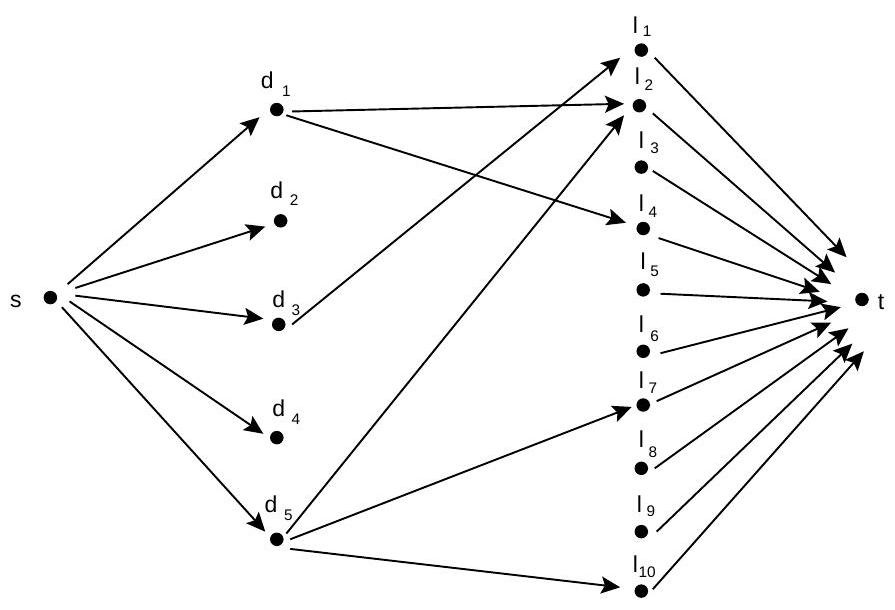
\includegraphics[max width=\textwidth, center]{2025_09_05_aa5f7b8425e7dd302062g-29}

Sea $x$ un flujo óptimo en $G_{u v}$. Para cada $1 \leq i \leq m, 1 \leq j \leq n$ sean $x_{s i}=x_{s d_{i}}$ y $x_{j t}=x_{l_{j} t}$ y, para cada $(i, j) \in \mathcal{A}$, sea $x_{i j}=x_{d_{i} l_{j}}$.\\
Notemos que valor de $x=\sum_{i=1}^{m} x_{s i} \leq \sum_{i=1}^{m} a_{i}$ ya que $x_{s i} \leq a_{i}$ para todo $i$.\\
Además

$$
\text { valor de } x=\sum_{i=1}^{m} x_{s i}=\sum_{i} x\left(V, d_{i}\right)=\sum_{i} x\left(d_{i}, V\right)=\sum_{(i, j) \in \mathcal{A}} x_{i j}
$$

Luego, $\sum_{(i, j) \in \mathcal{A}} x_{i j}=$ valor de $x \leq \sum_{i=1}^{m} a_{i}$.\\
Si valor de $x=\sum_{i=1}^{m} a_{i}$, tomando $x_{i j}=0$ para todo $(i, j) \notin \mathcal{A}(1 \leq i \leq m, 1 \leq j \leq n)$ se tiene que $\left(x_{i j}\right)$ es una solución óptima de $(\mathrm{P})$. En efecto, si valor de $x=\sum_{i=1}^{m} a_{i}$, entonces $\sum_{(i, j) \in \mathcal{A}} x_{i j}=\sum_{i=1}^{m} a_{i}$.\\
Luego, tomando $x_{i j}=0$ para todo $(i, j) \notin \mathcal{A}(1 \leq i \leq m, 1 \leq j \leq n)$, se tiene que

$$
\sum_{i, j} x_{i j}=\sum_{(i, j) \in \mathcal{A}} x_{i j}=\sum_{i=1}^{m} a_{i}
$$

Además,

$$
\begin{aligned}
\sum_{j=1}^{n} x_{i j} & =\sum_{j /(i, j) \in \mathcal{A}} x_{i j}=x_{s i} \leq a_{i} \\
\sum_{i=1}^{m} x_{i j} & =\sum_{i /(i, j) \in \mathcal{A}} x_{i j}=x_{j t} \leq b_{j} \\
x & \geq 0
\end{aligned}
$$

Luego, como $\sum_{i, j} x_{i j}=\sum_{i} a_{i}=\sum_{j} b_{j}$ entonces debe ser

$$
\sum_{j=1}^{n} x_{i j}=a_{i} \quad \text { у } \quad \sum_{i=1}^{m} x_{i j}=b_{j}
$$

(ya que si para algún $i$ fuese $\sum_{j=1}^{n} x_{i j}<a_{i}$ o para algún $j$ fuese $\sum_{i=1}^{m} x_{i j}<b_{j}$ entonces $\sum_{i, j} x_{i j}<\sum_{i=1}^{m} a_{i}=\sum_{j=1}^{n} b_{j}$ ).\\
Luego, $\left(x_{i j}\right)$ es una solución factible de $(\mathrm{P})$ que satisface $x_{i j}=0$ para todo $(i, j) \notin \mathcal{A}$, es decir, $x_{i j}=0$ para todo $(i, j)$ tal que $c_{i j}-\left(u_{i}+v_{j}\right)>0$, de donde $\left[c_{i j}-\left(u_{i}+v_{j}\right)\right] x_{i j}=0$. Entonces, $x$ y $(u, v)$ son soluciones factibles de (P) y (D) respectivamente que satisfacen la condición de holgura complementaria. Por lo tanto, $x$ es un óptimo de $(\mathrm{P})$ (y $(u, v)$ lo es de (D)).\\
Supongamos ahora que valor de $x<\sum_{i=1}^{m} a_{i}$\\
Sea $\partial B$ el mínimo corte correspondiente al flujo óptimo $x$ y sean $I=\left\{i / d_{i} \in B\right\}$ y $J=\left\{j / l_{j} \in B\right\}$. Como las flechas $\left(d_{i}, l_{j}\right)$ correspondientes a los $(i, j) \in \mathcal{A}$ tienen capacidad infinita entonces ninguna de ellas pertenece al corte $\partial B$ ya que

$$
\text { capacidad de } \partial B=\text { valor de } x<\sum_{i} a_{i}<\infty
$$

Luego, como $s \in B$ y $t \notin B$ se tiene que

$$
\partial B=\left\{\left(s, d_{i}\right) / i \notin I\right\} \cup\left\{\left(l_{j}, t\right) / j \in J\right\}
$$

de donde la capacidad del corte $\partial B$ es

$$
\sum_{i \notin I} a_{i}+\sum_{j \in J} b_{j}
$$

Como la capacidad de $\partial B$ es igual al valor de $x$ entonces

$$
\sum_{i \notin I} a_{i}+\sum_{j \in J} b_{j}=\text { valor de } x<\sum_{i} a_{i}=\sum_{j} b_{j}
$$

de donde

$$
\sum_{j \in J} b_{j}<\sum_{i=1}^{m} a_{i}-\sum_{i \notin I} a_{i}
$$

y

$$
\sum_{i \notin I} a_{i}<\sum_{j=1}^{n} b_{j}-\sum_{j \in J} b_{j}
$$

es decir,

$$
\sum_{j \in J} b_{j}<\sum_{i \in I} a_{i}
$$

y

$$
\sum_{i \notin I} a_{i}<\sum_{j \notin J} b_{j}
$$

Ahora construímos una nueva solución factible $(\bar{u}, \bar{v})$ de (D) tal que

$$
\sum_{i=1}^{m} \bar{u}_{i} a_{i}+\sum_{j=1}^{n} \bar{v}_{j} b_{j}>\sum_{i=1}^{m} u_{i} a_{i}+\sum_{j=1}^{n} v_{j} b_{j}
$$

(es decir, una nueva solución factible de ( D ) con un valor mayor del funcional) y, a partir del conjunto $\mathcal{A}^{\prime}=\left\{(i, j) / c_{i j}-\left(\bar{u}_{i}+\bar{v}_{j}\right)=0\right\}$, construímos el grafo $G_{\overline{u v}}=\left(V, E^{\prime}\right)$, tomando $V=X \cup Y \cup\{s, t\}$ y $E^{\prime}=\left\{\left(d_{i}, l_{j}\right) /(i, j) \in \mathcal{\mathcal { A } ^ { \prime }}\right\} \cup\left\{\left(s, d_{i}\right) / 1 \leq i \leq m\right\} \cup\left\{\left(l_{j}, t\right) / 1 \leq j \leq n\right\}$.\\
Si se verifica que valor de $\bar{x}=\sum_{i=1}^{m} a_{i}$ para un flujo óptimo $\bar{x}$ del grafo $G_{\overline{u v}}$, tomando $\bar{x}_{i j}=0$ para $(i, j) \notin \mathcal{A}^{\prime}$ tendríamos una solución óptima de $(\mathrm{P})$. En caso contrario, repetimos el procedimiento.\\
Veamos ahora cómo construír $(\bar{u}, \bar{v})$.\\
Sean

$$
\bar{u}_{i}=\left\{\begin{array}{ll}
u_{i}+\delta & \text { si } i \in I \\
u_{i}-\delta & \text { si } i \notin I
\end{array} \quad \bar{v}_{j}= \begin{cases}v_{j}-\delta & \text { si } j \in J \\
v_{j}+\delta & \text { si } j \notin J\end{cases}\right.
$$

donde $\delta>0$ será elegido de manera que ( $\bar{u}, \bar{v}$ ) sea una solución factible de (D). Notemos que cualquiera sea $\delta>0$ el valor del funcional en la nueva solución $(\bar{u}, \bar{v})$ será mayor que el valor del funcional en $(u, v)$. En efecto, como

$$
\sum_{j \in J} b_{j}<\sum_{i \in I} a_{i} \quad \text { у } \quad \sum_{i \notin I} a_{i}<\sum_{j \notin J} b_{j}
$$

se tiene

$$
\begin{aligned}
& \sum_{i=1}^{m} \bar{u}_{i} a_{i}+\sum_{j=1}^{n} \bar{v}_{j} b_{j}= \\
= & \sum_{i \in I}\left(u_{i}+\delta\right) a_{i}+\sum_{i \notin I}\left(u_{i}-\delta\right) a_{i}+ \\
+ & \sum_{j \in J}\left(v_{j}-\delta\right) b_{j}+\sum_{j \notin J}\left(v_{j}+\delta\right) b_{j}= \\
= & \sum_{i=1}^{m} u_{i} a_{i}+\sum_{j=1}^{n} v_{j} b_{j}+\delta(\underbrace{\sum_{i \in I} a_{i}-\sum_{j \in J} b_{j}}_{>0})+\delta(\underbrace{\sum_{j \notin J} b_{j}-\sum_{i \notin I} a_{i}}_{>0})> \\
> & \sum_{i=1}^{m} u_{i} a_{i}+\sum_{j=1}^{n} v_{j} b_{j}
\end{aligned}
$$

Veamos ahora cuál es el $\delta$ que nos sirve. Queremos que valga

$$
\bar{u}_{i}+\bar{v}_{j} \leq c_{i j}
$$

Si $i \notin I$ entonces

$$
\bar{u}_{i}+\bar{v}_{j}=u_{i}-\delta+v_{j} \pm \delta \leq u_{i}+v_{j} \leq c_{i j}
$$

Lo mismo ocurre si $j \in J$. Por lo tanto basta considerar el caso $i \in I, j \notin J$ donde debe verificarse que $u_{i}+v_{i}+2 \delta \leq c_{i j}$.\\
Observemos que si $i \in I$ y $j \notin J$ entonces $(i, j) \notin \mathcal{A}$. En efecto, si $(i, j) \in \mathcal{A}$ entonces la rama ( $d_{i}, l_{j}$ ) sería una rama de $G_{u v}$. Pero $I=\left\{i / d_{i} \in B\right\}$ y $J=\left\{j / l_{j} \in B\right\}$. Luego, como $i \in I$ y $j \notin J$ entonces $d_{i} \in B$ y $l_{j} \notin B$, de donde ( $d_{i}, l_{j}$ ) sería una rama de $G_{u v}$ que pertenecería al corte $\partial B$, cosa que no puede ocurrir ya que esta rama tiene capacidad infinita. Por lo tanto $(i, j) \notin \mathcal{A}$ con lo cual $u_{i}+v_{j}<c_{i j}$. Tomando

$$
\delta=\min \left\{\frac{c_{i j}-\left(u_{i}+v_{j}\right)}{2} / i \in I, j \notin J\right\}
$$

entonces se verifica que $\delta>0$ y $u_{i}+v_{i}+2 \delta \leq c_{i j}$ para todo $i \in I, j \notin J$ y se tiene que

$$
\bar{u}_{i}+\bar{v}_{j} \leq c_{i j} \quad \forall i, j
$$

Notemos que existen $i \in I$ y $j \notin J$ (es decir, $\left\{\frac{c_{i j}-\left(u_{i}+v_{j}\right)}{2} / i \in I, j \notin J\right\}$ es no vacío) pues si $I=\emptyset$ o $J=\{1,2, \ldots, n\}$ entonces se tendría que valor de $x=\sum_{i} a_{i}$. En efecto, si $I=\emptyset$ entonces, para todo $i$, $d_{i} \notin B$ de donde, para todo $i$, no existe camino aumentativo de $s$ a $d_{i}$. Luego, debe ser $x_{s i}=a_{i}$ para todo $i \mathrm{y}$, por lo tanto, valor de $x=\sum_{i} x_{s i}=\sum_{i} a_{i}$. Análogamente, si $J=\{1,2, \ldots, n\}$ entonces, para todo $j$, $l_{j} \in B$, es decir, para todo $j$ existe un camino aumentativo a $l_{j} \mathrm{y}$, como $t \notin B$ entonces ese camino seguido de la rama ( $l_{j}, t$ ) no puede ser un camino aumentativo. Por lo tanto, para todo $j$ debe ser $x_{j t}=b_{j}$, con lo cual valor de $x=\sum_{i} x_{s i}=\sum_{j} x_{j t}=\sum_{j} b_{j}=\sum_{i} a_{i}$.\\
Por último observemos que, para hallar un flujo óptimo en $G_{\overline{u v}}$, puede aplicarse el algoritmo de FordFulkerson utilizando como flujo factible inicial al flujo $x^{\prime}$ en $G_{\overline{u v}}$ definido por

$$
\begin{aligned}
x_{s i}^{\prime} & =x_{s i} \quad \forall i \\
x_{j t}^{\prime} & =x_{j t} \quad \forall j \\
x_{i j}^{\prime} & =x_{i j} \quad \forall(i, j) \in \mathcal{A}^{\prime} \cap \mathcal{A} \\
x_{i j}^{\prime} & =0 \quad \forall(i, j) \in \mathcal{A}^{\prime}-\mathcal{A}
\end{aligned}
$$

En efecto, basta ver que $x^{\prime}$ es un flujo factible en $G_{\overline{u v}}$.\\
Notemos que $x_{i j}=0$ para todo $(i, j) \in \mathcal{A}-\mathcal{A}^{\prime}$. En efecto, supongamos que $(i, j) \in \mathcal{A}-\mathcal{A}^{\prime}$. Si $i \in I$ y $j \in J$ o si $i \notin I$ y $j \notin J$ entonces $c_{i j}-\left(\bar{u}_{i}+\bar{v}_{j}\right)=c_{i j}-\left(u_{i}+v_{j}\right)$, lo que no puede ocurrir ya que $c_{i j}-\left(\bar{u}_{i}+\bar{v}_{j}\right) \neq 0$ pues $(i, j) \notin \mathcal{A}^{\prime}$ y $c_{i j}-\left(u_{i}+v_{j}\right)=0$ pues $(i, j) \in \mathcal{A}$. Y si $i \in I$ y $j \notin J$ entonces $d_{i} \in B$ y $l_{j} \notin B$ y, como ( $d_{i}, l_{j}$ ) es una rama de $G_{u v}$ pues $(i, j) \in \mathcal{A}$ entonces se tendría que $\left(d_{i}, l_{j}\right) \in \partial B$, cosa que tampoco puede ocurrir ya que $\partial B$ no contiene ramas de capacidad infinita. Luego se tiene que $i \notin I$ y $j \in J$, de donde $d_{i} \notin B$ y $l_{j} \in B$. Por lo tanto, $\left(d_{i}, l_{j}\right)$ es una rama de $G_{u v}$ (pues $(i, j) \in \mathcal{A}$ ) y además $\left(d_{i}, l_{j}\right) \in \partial \bar{B}$. Como valor de $x=$ capacidad de $\partial B$ ya que $x$ es un flujo máximo en $G_{u v}$ y $\partial B$ es el correspondiente mínimo corte, por la observación 4.5. se tiene que $x_{i j}=0 \forall(i, j) \in \partial \bar{B}$. Luego, $x_{i j}=0$ para todo $(i, j) \in \mathcal{A}-\mathcal{A}^{\prime}$.\\
Luego, como $x_{i j}^{\prime}=0$ para todo $(i, j) \in \mathcal{A}^{\prime}-\mathcal{A}, x_{i j}^{\prime}=x_{i j}$ para todo $(i, j) \in \mathcal{A}^{\prime} \cap \mathcal{A}, x_{i j}=0$ para todo $(i, j) \in \mathcal{A}-\mathcal{A}^{\prime}$ y $x$ es un flujo factible en $G_{u v}$, se tiene

$$
\begin{aligned}
x^{\prime}\left(d_{i}, V\right) & =\sum_{j /(i, j) \in \mathcal{A}^{\prime}} x_{i j}^{\prime}=\sum_{j /(i, j) \in \mathcal{A}^{\prime} \cap \mathcal{A}} x_{i j}^{\prime}+\sum_{j /(i, j) \in \mathcal{A}^{\prime}-\mathcal{A}} x_{i j}^{\prime}=\sum_{j /(i, j) \in \mathcal{A}^{\prime} \cap \mathcal{A}} x_{i j}^{\prime}= \\
& =\sum_{j /(i, j) \in \mathcal{A}^{\prime} \cap \mathcal{A}} x_{i j}=\sum_{j /(i, j) \in \mathcal{A}^{\prime} \cap \mathcal{A}} x_{i j}+\sum_{j /(i, j) \in \mathcal{A}-\mathcal{A}^{\prime}} x_{i j}= \\
& =\sum_{j /(i, j) \in \mathcal{A}} x_{i j}=x\left(d_{i}, V\right)=x\left(V, d_{i}\right)=x_{s i}=x_{s i}^{\prime}=x^{\prime}\left(V, d_{i}\right)
\end{aligned}
$$

y

$$
\begin{aligned}
x^{\prime}\left(V, l_{j}\right) & =\sum_{i /(i, j) \in \mathcal{A}^{\prime}} x_{i j}^{\prime}=\sum_{i /(i, j) \in \mathcal{A}^{\prime} \cap \mathcal{A}} x_{i j}^{\prime}+\sum_{i /(i, j) \in \mathcal{A}^{\prime}-\mathcal{A}} x_{i j}^{\prime}=\sum_{i /(i, j) \in \mathcal{A}^{\prime} \cap \mathcal{A}} x_{i j}^{\prime}= \\
& =\sum_{i /(i, j) \in \mathcal{A}^{\prime} \cap \mathcal{A}} x_{i j}=\sum_{i /(i, j) \in \mathcal{A}^{\prime} \cap \mathcal{A}} x_{i j}+\sum_{i /(i, j) \in \mathcal{A}-\mathcal{A}^{\prime}} x_{i j}= \\
& =\sum_{i /(i, j) \in \mathcal{A}} x_{i j}=x\left(V, l_{j}\right)=x\left(l_{j}, V\right)=x_{j t}=x_{j t}^{\prime}=x^{\prime}\left(l_{j}, V\right)
\end{aligned}
$$

Por lo tanto, $x^{\prime}$ es un flujo factible en $G_{\overline{u v}}$ como queríamos demostrar.

\section*{Descripción del algoritmo primal-dual para resolver el problema del transporte.}
\begin{enumerate}
  \item Tomar una solución factible inicial $(u, v)$ cualquiera de $(\mathrm{D})$, por ejemplo, $u_{i}=0, v_{j}=\min _{i} c_{i j}$. Hallar $\mathcal{A}=\left\{(i, j) / c_{i j}-\left(u_{i}+v_{j}\right)=0\right\}$. Inicializar $x^{\prime}=0$.
  \item Construír el grafo $G_{u v}=(V, E)$ con vértices $V=\left\{d_{1}, d_{2}, \ldots, d_{m}\right\} \cup\left\{l_{1}, l_{2}, \ldots, l_{n}\right\} \cup\{s, t\}$ y ramas $E=\left\{\left(d_{i}, l_{j}\right) /(i, j) \in \mathcal{A}\right\} \cup\left\{\left(s, d_{i}\right) / 1 \leq i \leq m\right\} \cup\left\{\left(l_{j}, t\right) / 1 \leq j \leq n\right\}$. Asignar capacidad $a_{i}$ a las ramas $\left(s, d_{i}\right)$, capacidad $b_{j}$ a las ramas $\left(l_{j}, t\right)$ y capacidad infinita a las ramas $\left.\left(d_{i}, l_{j}\right)((i, j) \in \mathcal{A})\right)$.
  \item Hallar un flujo $x$ de valor máximo en el grafo $G_{u v}$, aplicando el de Ford-Fulkerson con $x^{\prime}$ como flujo factible inicial.\\
Si valor de $x=\sum_{i=1}^{m} a_{i} \operatorname{STOP}\left(\right.$ en este caso tomando $x_{i j}=x_{d_{i} l_{j}}$ para $(i, j) \in \mathcal{A}$ y $x_{i j}=0$ para $(i, j) \notin \mathcal{A}$ se obtiene una solución óptima del problema).
  \item Sea $B$ el último conjunto construído por el algoritmo de Ford-Fulkerson (es decir, el que define el mínimo corte correspondiente al flujo óptimo $x$ hallado en el paso 3 . cuyos elementos son $s$ y todos los vértices que pueden ser alcanzados por un camino aumentativo de $x$ ).\\
Hallar $I=\left\{i / d_{i} \in B\right\}, J=\left\{j / l_{j} \in B\right\}$ y $\delta=\min \left\{\frac{c_{i j}-\left(u_{i}+v_{j}\right)}{2} / i \in I, j \notin J\right\}$. Poner
\end{enumerate}

$$
\bar{u}_{i}=\left\{\begin{array}{ll}
u_{i}+\delta & \text { si } i \in I \\
u_{i}-\delta & \text { si } i \notin I
\end{array} \quad \bar{v}_{j}= \begin{cases}v_{j}-\delta & \text { si } j \in J \\
v_{j}+\delta & \text { si } j \notin J\end{cases}\right.
$$

y hallar $\mathcal{A}^{\prime}=\left\{(i, j) / c_{i j}-\left(\bar{u}_{i}+\bar{v}_{j}\right)=0\right\}$.\\
Actualizar $x^{\prime}$ en la forma

$$
\begin{aligned}
x_{s i}^{\prime} & =x_{s i} \quad \forall i \\
x_{j t}^{\prime} & =x_{j t} \quad \forall j \\
x_{i j}^{\prime} & =x_{i j} \quad \forall(i, j) \in \mathcal{A}^{\prime} \cap \mathcal{A} \\
x_{i j}^{\prime} & =0 \quad \forall(i, j) \in \mathcal{A}^{\prime}-\mathcal{A}
\end{aligned}
$$

\begin{enumerate}
  \setcounter{enumi}{4}
  \item Reemplazar $(u, v)$ por $(\bar{u}, \bar{v})$, reemplazar $\mathcal{A}$ por $\mathcal{A}^{\prime}$ e ir a 2 .
\end{enumerate}

\section*{Convergencia del algoritmo para el problema del transporte.}
Probaremos ahora que el algoritmo que acabamos de describir termina en un número finito de pasos y que, cuando lo hace, se tiene una solución ( $x_{i j}$ ) entera del problema del transporte. Recordemos que $a_{i} (1 \leq i \leq m)$ y $b_{j}(1 \leq j \leq n)$ son enteros positivos y notemos que en el paso 3 . de cada iteración del algoritmo hallamos un flujo factible $x$ en $G_{u v}$ que satisface valor de $x \leq \sum_{i=1}^{m} a_{i}$.\\
Notemos también que el máximo flujo $x$ hallado en cada iteración es entero. En efecto, por la observación 4.4., el máximo flujo $x$ obtenido en la primera iteración es entero ya que se obtiene aplicando el algoritmo de Ford-Fulkerson a un grafo cuyas ramas tienen capacidades enteras o infinitas y que satisface que las ramas\\
que salen de $s$ tienen capacidad entera, partiendo del flujo factible inicial $x^{\prime}=0$ que es entero. Supongamos ahora que el máximo flujo $x$ obtenido en la $k$-ésima iteración sea entero y veamos que esto también vale en la iteración $k+1$ : sea $\bar{x}$ el máximo flujo obtenido en la iteración $k+1$. Entonces, nuevamente por la observación 4.4., $\bar{x}$ es entero ya que se obtiene aplicando el algoritmo de Ford-Fulkerson a un grafo cuyas ramas tienen capacidades enteras o infinitas y que satisface que las ramas que salen de $s$ tienen capacidad entera, partiendo del flujo factible inicial $x^{\prime}$ que es entero pues $x^{\prime}$ está definido por

$$
\begin{aligned}
x_{s i}^{\prime} & =x_{s i} \quad \forall i \\
x_{j t}^{\prime} & =x_{j t} \quad \forall j \\
x_{i j}^{\prime} & =x_{i j} \quad \forall(i, j) \in \mathcal{A}^{\prime} \cap \mathcal{A} \\
x_{i j}^{\prime} & =0 \quad \forall(i, j) \in \mathcal{A}^{\prime}-\mathcal{A}
\end{aligned}
$$

y $x$ es entero por hipótesis inductiva.\\
Por otra parte, si $x$ es el máximo flujo obtenido en la $k$-ésima iteración y $\bar{x}$ es el máximo flujo obtenido en la iteración $k+1$, entonces se tiene que valor de $x \leq$ valor de $\bar{x}$, ya que valor de $x=$ valor de $x^{\prime}$ y $\bar{x}$ se obtiene partiendo del flujo inicial $x^{\prime}$. Además, si valor de $x<$ valor de $\bar{x}$ entonces $1+$ valor de $x \leq$ valor de $\bar{x}$, ya que valor de $x$ y valor de $\bar{x}$ son enteros. Veamos ahora qué sucede si valor de $x=$ valor de $\bar{x}$.\\
Sea $x$ el máximo flujo obtenido en la $k$-ésima iteración y sea $\bar{x}$ es el máximo flujo obtenido en la iteración $k+1$ y supongamos que valor de $x=$ valor de $\bar{x}$. Sean ( $u, v$ ) la solución factible del dual presente al iniciarse la $k$-ésima iteración, $\mathcal{A}=\left\{(i, j) / c_{i j}-\left(u_{i}+v_{j}\right)=0\right\}, \partial B$ el mínimo corte correspondiente al máximo flujo $x$ en $G_{u v}$ y sean $I=\left\{i / d_{i} \in B\right\}, J=\left\{j / l_{j} \in B\right\}$ y $\delta=\min \left\{\frac{c_{i j}-\left(u_{i}+v_{j}\right)}{2} / i \in I, j \notin J\right\}$. Sea $(\bar{u}, \bar{v})$ la solución factible del dual presente al iniciarse la iteración $k+1$, es decir, la definida por

$$
\bar{u}_{i}=\left\{\begin{array}{ll}
u_{i}+\delta & \text { si } i \in I \\
u_{i}-\delta & \text { si } i \notin I
\end{array} \quad \bar{v}_{j}= \begin{cases}v_{j}-\delta & \text { si } j \in J \\
v_{j}+\delta & \text { si } j \notin J\end{cases}\right.
$$

y sean $\mathcal{A}^{\prime}=\left\{(i, j) / c_{i j}-\left(\bar{u}_{i}+\bar{v}_{j}\right)=0\right\}, \partial B^{\prime}$ el mínimo corte correspondiente al máximo flujo $\bar{x}$ en $G_{\overline{u v}}$, $I^{\prime}=\left\{i / d_{i} \in B^{\prime}\right\}$ y $J^{\prime}=\left\{j / l_{j} \in B^{\prime}\right\}$.\\
Como valor de $x=$ valor de $\bar{x}$ entonces el flujo inicial $x^{\prime}$ en $G_{\overline{u v}}$ definido por

$$
\begin{aligned}
x_{s i}^{\prime} & =x_{s i} \quad \forall i \\
x_{j t}^{\prime} & =x_{j t} \quad \forall j \\
x_{i j}^{\prime} & =x_{i j} \quad \forall(i, j) \in \mathcal{A}^{\prime} \cap \mathcal{A} \\
x_{i j}^{\prime} & =0 \quad \forall(i, j) \in \mathcal{A}^{\prime}-\mathcal{A}
\end{aligned}
$$

debe ser óptimo ya que

$$
\text { valor de } x^{\prime}=\sum_{i} x_{s i}^{\prime}=\sum_{i} x_{s i}=\text { valor de } x=\text { valor de } \bar{x}
$$

Por lo tanto $\bar{x}=x^{\prime}$ ya que $\bar{x}$ se obtiene aplicando el algoritmo de Ford-Fulkerson utilizando como flujo inicial el flujo $x^{\prime}$ que ya es óptimo. Luego, los elementos de $B^{\prime}$ son $s$ y todos los vértices que pueden ser alcanzados por un camino aumentativo de $x^{\prime}$.

Afirmación: $B \subseteq B^{\prime}$\\
Demostración: Sea $w \in B, w \neq s$. Entonces, como $\partial B$ es el mínimo corte correspondiente al flujo óptimo $x$ en $G_{u v}$, existe en $G_{u v}$ un camino $\mathcal{P}$ aumentativo de $x$ de $s$ a $w$. Probaremos que este camino es un camino aumentativo de $x^{\prime}$ de $s$ a $w$ en $G_{\overline{u v}}$, de donde resulta que $w \in B^{\prime}$.

En efecto, si $\left(d_{i}, l_{j}\right)$ es una rama de $\mathcal{P}$ entonces $(i, j) \in \mathcal{A}$ (pues ( $d_{i}, l_{j}$ ) es una rama de $G_{u v}$ ) y además $i \in I$ y $j \in J$ (pues la parte $\mathcal{P}$ de $s$ hasta $d_{i}$ es un camino aumentativo de $x$ en $G_{u v}$ de $s$ a $d_{i}$, con lo cual $d_{i} \in B$ y la parte de $\mathcal{P}$ de $s$ hasta $l_{j}$ es un camino aumentativo de $x$ en $G_{u v}$ de $s$ a $l_{j}$, con lo cual $l_{j} \in B$ ). Luego, $\bar{u}_{i}=u_{i}+\delta$ y $\bar{v}_{j}=v_{j}-\delta$, de donde $c_{i j}-\left(\bar{u}_{i}+\bar{v}_{j}\right)=c_{i j}-\left(u_{i}+v_{j}\right)=0$ pues $(i, j) \in \mathcal{A}$. Por lo tanto $(i, j) \in \mathcal{A}^{\prime}$. Entonces $\left(d_{i}, l_{j}\right)$ es una rama de $G_{\overline{u v}}$ y además vale que $x_{i j}^{\prime}=x_{i j}$ ya que $(i, j) \in \mathcal{A} \cap \mathcal{A}^{\prime}$.\\
Además, si $\left(s, d_{i}\right)$ es una rama de $\mathcal{P}$ entonces es claro que también es una rama de $G_{\overline{u v}}$ y vale $x_{s i}^{\prime}=x_{s i}$.\\
Como $\mathcal{P}$ no puede contener ramas del tipo ( $l_{j}, t$ ) ya que $t \notin B$ esto muestra que $\mathcal{P}$ es un camino aumentativo de $x^{\prime}$ de $s$ a $w$ en $G_{\overline{u v}}$ como queríamos probar.\\
Luego, $B \subseteq B^{\prime}$ como habíamos afirmado y, por lo tanto, se tiene que $I \subseteq I^{\prime}$ y $J \subseteq J^{\prime}$.\\
Recordemos que $\delta=\min \left\{\frac{c_{i j}-\left(u_{i}+v_{j}\right)}{2} / i \in I, j \notin J\right\}$. Sean $i_{0} \in I$ y $j_{0} \notin J$ tales que $\delta=\frac{c_{i_{0} j_{0}}-\left(u_{i_{0}}+v_{j_{0}}\right)}{2}$. Luego

$$
c_{i_{0} j_{0}}-\left(\bar{u}_{i_{0}}+\bar{v}_{j_{0}}\right)=c_{i_{0} j_{0}}-\left(u_{i_{0}}+\delta+v_{j_{0}}+\delta\right)=c_{i_{0} j_{0}}-\left(u_{i_{0}}+v_{j_{0}}\right)-2 \delta=0
$$

de donde resulta que $\left(i_{0}, j_{0}\right) \in \mathcal{A}^{\prime}$, es decir, $\left(d_{i_{0}}, l_{j_{0}}\right)$ es una rama de $G_{\overline{u v}}$. Como esta rama tiene capacidad infinita entonces no puede pertenecer al corte $\delta B^{\prime}$ que tiene capacidad finita y como $d_{i_{0}} \in B^{\prime}$ (pues $i \in I \subseteq I^{\prime}$ ) entonces $l_{j_{0}} \in B^{\prime}$, es decir, $j_{0} \in J^{\prime}$. Como $j_{0} \notin J$, esto muestra que $J \subseteq J^{\prime}$ y $J \neq J^{\prime}$. Por lo tanto $\# J<\# J^{\prime}$ de donde $\# J^{\prime} \geq \# J+1$.\\
Por otra parte, como valor de $x=$ valor de $\bar{x}$ entonces

$$
\sum_{i \notin I^{\prime}} a_{i}+\sum_{j \in J^{\prime}} b_{j}=\text { valor de } \bar{x}=\text { valor de } x=\sum_{i \notin I} a_{i}+\sum_{j \in J} b_{j}
$$

si fuese $I=I^{\prime}$ entonces se tendría que

$$
\sum_{j \in J} b_{j}=\sum_{j \in J^{\prime}} b_{j}=\sum_{j \in J} b_{j}+\sum_{j \in J^{\prime}-J} b_{j}>\sum_{j \in J} b_{j}
$$

pues $J \subseteq J^{\prime}, J \neq J^{\prime}$ y $b_{j}>0$ para todo $j=1,2, \ldots, n$. Luego, $I \neq I^{\prime}$ y, como $I \subseteq I^{\prime}$ entonces $\# I^{\prime} \geq \# I+1$.\\
En resumen, hemos probado que el máximo flujo $x$ obtenido en la $k$-ésima iteración del algoritmo y el máximo flujo $\bar{x}$ obtenido en la iteración $k+1$ siempre satisfacen valor de $\bar{x} \geq$ valor de $x$, que si valor de $\bar{x}>$ valor de $x$ entonces valor de $\bar{x} \geq 1+$ valor de $x$ (es decir, si el valor del flujo aumenta, lo hace en por lo menos una unidad) y que si en cambio valor de $x=$ valor de $\bar{x}$ (es decir, si el valor del flujo no aumenta en una iteración) entonces los conjuntos $I$ y $J$ calculados por el algoritmo en el paso 4 de la iteración $k+1$ tiene al menos un elemento más cada uno que los calculados en la iteración $k$-ésima.

Conclusión: El valor del flujo sólo puede permanecer constante en a lo sumo $r=\min \{m, n\}$ iteraciones sucesivas, ya que el cardinal del conjunto $I$ calculado por el algoritmo en el paso 4 es siempre menor o igual que $m$ y el del conjunto $J$ es siempre menor o igual que $n$. Por lo tanto, cada $r+1$ iteraciones el valor del flujo necesariamente debe aumentar en al menos una unidad. Dado que el valor del flujo en cualquier iteración está acotado por $\sum_{i} a_{i}$ entonces el algoritmo termina en a lo sumo $(r+1) \sum_{i} a_{i}$ iteraciones, donde $r=\min \{m, n\}$.


\end{document}